\cotefile{134-8}
\scanpage{43}
\mspage{42}

\[
(f,i)\qquad (f,i')
\]

\diagram{\begin{tikzcd}[column sep=large]
x \arrow[r] \arrow[dr] & y \\
& \bar y \arrow[u]
\end{tikzcd}}

\diagram{\begin{tikzcd}[column sep=large,row sep=small]
y\amalg y \arrow[r,"{(i,i')}"] \arrow[d] & \bar y \arrow[dd,"\unsure{a|\alpha}"] \arrow[ddr,"\alpha"] & \\
c_y \arrow[d] & & \\
\unsure{y|c} \arrow[u,bend left] \arrow[r,Rightarrow] \arrow[rr,bend right=28,"1"'] & z \arrow[r] & y
\end{tikzcd}
\qquad
\begin{tikzcd}[column sep=large]
y\amalg y \arrow[r,"{(i,i')}"] \arrow[d] & \bar y \arrow[d,squiggly] \arrow[dr] & \\
c_y \arrow[r,Rightarrow] \arrow[rr] & \deleted{\unsure{y'}} & y
\end{tikzcd}}

\begin{center}
\rotatebox{180}{\begin{tabular}{l}
\texttt{3.04.01 PM 25 AUG 82 R6.PR1 SYS JES2 JOB 421 START A****}\\
\texttt{3.04.01 PM 25 AUG 82 R6.PR1 SYS JES2 JOB 421 START A****}\\
\texttt{3.04.01 PM 25 AUG 82 R6.PR1 SYS JES2 JOB 421 START A****}\\
\texttt{3.04.01 PM 25 AUG 82 R6.PR1 SYS JES2 JOB 421 START A****}\\
\texttt{3.04.01 PM 25 AUG 82 R6.PR1 SYS JES2 JOB 421 START A****}\\
\texttt{3.04.01 PM 25 AUG 82 R6.PR1 SYS JES2 JOB 421 START A****}
\end{tabular}}
\end{center}

\diagram{\rotatebox{180}{\begingroup\setlength{\arraycolsep}{\tabcolsep}$\begin{array}{llll}
\text{\texttt{PPP}}  & \text{\texttt{HH\phantom{HHHHHHHH}HH}} & \text{\texttt{IIIIIIIIII}} & \text{\texttt{\phantom{2}2222222222\phantom{2}}}\\
\text{\texttt{PPPP}} & \text{\texttt{HH\phantom{HHHHHHHH}HH}} & \text{\texttt{IIIIIIIIII}} & \text{\texttt{222222222222}}\\
\text{\texttt{\phantom{PP}PP}} & \text{\texttt{HH\phantom{HHHHHHHH}HH}} & \text{\texttt{\phantom{IIII}II}} & \text{\texttt{22\phantom{22222222}22}}\\
\text{\texttt{\phantom{PP}PP}} & \text{\texttt{HH\phantom{HHHHHHHH}HH}} & \text{\texttt{\phantom{IIII}II}} & \text{\texttt{\phantom{2222222222}22}}\\
\text{\texttt{\phantom{PP}PP}} & \text{\texttt{HH\phantom{HHHHHHHH}HH}} & \text{\texttt{\phantom{IIII}II}} & \text{\texttt{\phantom{2222222222}22}}\\
\text{\texttt{PPPP}} & \text{\texttt{HHHHHHHHHHHH}} & \text{\texttt{\phantom{IIII}II}} & \text{\texttt{\phantom{222222222}22}}\\
\text{\texttt{PPP}} & \text{\texttt{HHHHHHHHHHHH}} & \text{\texttt{\phantom{IIII}II}} & \text{\texttt{\phantom{2222222}22}}\\
& \text{\texttt{HH\phantom{HHHHHHHH}HH}} & \text{\texttt{\phantom{IIII}II}} & \text{\texttt{\phantom{22222}22}}\\
& \text{\texttt{HH\phantom{HHHHHHHH}HH}} & \text{\texttt{\phantom{IIII}II}} & \text{\texttt{\phantom{222}22}}\\
& \text{\texttt{HH\phantom{HHHHHHHH}HH}} & \text{\texttt{\phantom{IIII}II}} & \text{\texttt{\phantom{2}22}}\\
& \text{\texttt{HH\phantom{HHHHHHHH}HH}} & \text{\texttt{IIIIIIIIII}} & \text{\texttt{222222222222}}\\
& \text{\texttt{HH\phantom{HHHHHHHH}HH}} & \text{\texttt{IIIIIIIIII}} & \text{\texttt{222222222222}}
\end{array}$\endgroup}}

\diagram{\begin{tikzcd}
\bar y \arrow[d] & \\
y \arrow[u,bend right=45] \arrow[u,bend right=60] & \unsure{\alpha}
\end{tikzcd}}

\diagram{\rotatebox{90}{\begin{tikzcd}[ampersand replacement=\&]
x \arrow[dr,"f"'] \& \unsure{\bar{\bar y}|\bar y} \arrow[d,shift left,"\unsure{i'}"] \arrow[dr,"\unsure{u}"] \& \unsure{y} \arrow[d,"i"] \\
\& \bar y \arrow[u,shift left] \& \bar y
\end{tikzcd}}}
\[
\rotatebox{90}{$[i]^{-1}[\unsure{u}]=[i']^{-1}$}
\]
\scanpage{44}

\diagram{\begin{tikzcd}[column sep=large]
\unsure{x} \arrow[dr,"1"'] & y \arrow[l,"1"'] \arrow[d,"i'"] \arrow[dr,Rightarrow,"i''"] & \\
& \unsure{x} \arrow[r] \arrow[dr,leftrightarrow] & x \arrow[d] \\
& & x'
\end{tikzcd}}

\diagram{\begin{tikzcd}[column sep=large]
x \arrow[dr,no head,"f"'] & y \arrow[d,"i"] \arrow[dr,"g"] & z \arrow[d] \\
& \bar y \arrow[r,dashed,"\unsure{i}"'] \arrow[dr] \arrow[dr,dashed,shift left=3pt] & \bar z \arrow[d] \\
& & \unsure{-}
\end{tikzcd}
\qquad
\begin{tikzcd}
y \arrow[d] \arrow[dr] & \\
{} & {}
\end{tikzcd}}

\mspage{43}
\scanpage{45}

\[
I\times a\xrightarrow[\mathrm{asph.}]{}\unsure{a}
\qquad
\underset{\begin{smallmatrix}\Vert\\J\end{smallmatrix}}{\mathbb Z^{(I)}}
\otimes\mathbb Z^{(\unsure{e|0})}\longrightarrow\mathbb Z^{(\unsure{e|0})}
\]

\diagram{\begin{tikzcd}
& I \\
e \arrow[ur] & e \arrow[u]
\end{tikzcd}}

\diagram{\begin{tikzcd}
\widehat A \arrow[r,no head] \arrow[d,"\mathrm{wh}"',"\deleted{\unsure{\mathbb Z}}"] & (\mathrm{Hot}) \arrow[d,"\uline{wh}"] \\
\widehat A_{ab} \arrow[r,"Lp_!"] & \mathrm D_{\unsure{\bullet}}(Ab)
\end{tikzcd}}

\[
\mathbb Z^{(e\amalg e)}\xrightarrow{\sim}\mathbb Z^{(e)}\times\mathbb Z^{(e)}
\]

\diagram{$\left\{\begin{gathered}
\begin{tikzcd}
\mathbb Z_{\mathcal M} \arrow[r,shift left] \arrow[r,shift right] & J \arrow[r] & \mathbb Z_{\mathcal M}
\end{tikzcd}\\[1em]
J\otimes x\longrightarrow x\qquad\text{ds }W
\end{gathered}\right.$}

\[
\mathbb Z_{\mathcal M}\times\mathbb Z_{\mathcal M}\longrightarrow J\;\text{---}
\]

\[
P\longrightarrow P\otimes_kP
\qquad
\begin{gathered}
\mathbb Z_P=\mathbb Z_{P^h}\\
\mathbb Z_Q=\mathbb Z_{Q^h}
\end{gathered}
\]

\diagram{$\left\{\begin{gathered}
\begin{tikzcd}
& J \arrow[dr] & \\
\mathbb Z_{\mathcal M}\times\mathbb Z_{\mathcal M} \arrow[ur,hook] \arrow[rr] & & \mathbb Z_{\mathcal M}
\end{tikzcd}\\[1em]
J\otimes x\longrightarrow x\qquad\text{équiv. faible}
\end{gathered}\right.$}

\diagram{\begin{tikzcd}
\Delta_1 \arrow[d,"p"] & \deleted{\unsure{p_!\mathbb Z}} & \\
{} & 0 \arrow[r] & 1
\end{tikzcd}}

\[
\operatorname{Add}(\Delta_1)\subset\widehat\Delta_{1\,ab}
=\text{Cat des diagrammes }L_1\longrightarrow L_0\quad\text{\uline{dans $Ab$}}
\]

\[
J^+\otimes x\qquad\deleted{\unsure{tot.}}\unsure{h.}\ \text{acyclique}
\qquad\forall x
\]

\[
\mathbb Z^{(1)}=\{\mathbb Z\xrightarrow{\mathrm{id}}\mathbb Z\}
\qquad
J\simeq\mathbb Z_{\mathcal M}+J^+
\]
\[
\mathbb Z^{(0)}=\{0\longrightarrow\mathbb Z\}
\qquad
\mathbb Z_{\mathcal M}\xrightarrow{\deleted{\unsure{\lambda}}}J^+
\qquad\lambda\ \text{injectif}
\]

\[
\mathbb Z_{\mathcal M}\subset J^+
\]

\noindent
$\operatorname{Add}(\Delta_1)=$ Catégorie des complexes
$0\mathbin{-}L_1\unsure{\mathbin{-}|\longrightarrow}L_0\mathbin{-}0$
de longueur \unsure{1|2}, avec
\inserted{$L_0,L_1,$}\deleted{$L_1,$}
$H_0(L_\bullet)$ \inserted{libres}\deleted{\unsure{f.g.}}\inserted{t.f.}
et $H_1(L_\bullet)=0$,

\noindent i.e.
\[
0\mathbin{-}L_1\longrightarrow L_0\longrightarrow H_0\mathbin{-}0
\]
avec $L_0,L_1$

\[
\left\{\begin{aligned}
\mathbb Z_{\mathcal M}\times\mathbb Z_{\mathcal M}&\longrightarrow J\\
(x,y)&\longmapsto(x+y,\lambda(y))\\
&\deleted{x+y=0}\\
(x,-x)&\longmapsto(0,\lambda(x))
\end{aligned}\right.
\]

\[
\boxed{\boxed{\begin{gathered}
\mathbb Z_{\mathcal M}\hookrightarrow J^+\\
J^+\otimes X\quad\deleted{\unsure{tot.}}\ \text{acyclique}\quad
\forall x\in\underline P
\end{gathered}}}
\]

\mspage{44}
\scanpage{46}

\[
\mathbb Z^{(i)}(j)=\mathbb Z^{(\operatorname{Hom}(j,i))}
=\begin{cases}\mathbb Z&\text{si }j\leq i\\0&\text{si }j>i\end{cases}
\]
\[
0\mathbin{-}\overset{i}{\mathbb Z}\longrightarrow\mathbb Z\longrightarrow\cdots
\mathbin{-}\overset{0}{\mathbb Z}\mathbin{-}0
\]

\figure{\begin{tikzpicture}\draw (0,0)--(8,0)--(8,2.2);\end{tikzpicture}}

\margin{$\varphi J(\qquad J$}

\[
\mathcal M=M^h
\]

1) $L_i\varphi(\mathbb Z_{\mathcal M})=0$ si $i>0$.

2) \deleted{$\exists J_{\mathcal M}^+$ tel que}
\[
\mathbb Z_{\mathcal M}\lhook\joinrel\xrightarrow{\alpha}J_{\mathcal M}^+
\quad\text{(mono) \inserted{dans $\mathcal M$} tel que}
\]
\[
L_i\varphi(J_{\mathcal M}^+\otimes x)\deleted{\text{est acyclique}}=0
\qquad\forall\ \text{\textcircled{\scriptsize$i\geq0$}},\ x\in\mathcal M.
\]

\[
\begin{gathered}
(L_i\varphi)(J\otimes_k a)=0\qquad\forall i\in\mathbb N,\ a\in M\\
\Updownarrow\qquad\forall i\in\mathbb N,\ a\in\mathcal M
\end{gathered}
\]

\[
0\mathbin{-}J\otimes L_\bullet\longrightarrow\mathbb Z^{(I)}\otimes L_\bullet
\mathbin{-}\deleted{\unsure{x}}L_\bullet\mathbin{-}0
\]

\deleted{\uline{NB} On peut prendre $J_{\mathcal M}^+=\mathbb Z_{\mathcal M}$}

\[
I\times X\mathbin{-}X
\]

\[
\underset{\begin{smallmatrix}\Vert\\\mathbb Z^{(e)}\times\mathbb Z^{(e)}\end{smallmatrix}}
{\mathbb Z^{(e\amalg e)}}\longrightarrow\mathbb Z
\]

\[
0\longrightarrow J\mathbin{-}\mathbb Z^{(I)}\longrightarrow\mathbb Z_{\widehat A}\mathbin{-}0
\]
\[
0\longrightarrow J\otimes F\mathbin{-}
\underbrace{\mathbb Z^{(I)}\otimes F}_{\deleted{\unsure{\mathbb Z^{(F)}}}\;F^{(I)}}
\mathbin{-}F\longrightarrow0
\]
\inserted{\deleted{est projectif.} \unsure{résolution} avec augmentation!!}

OK alors $F=\mathbb Z^{(X)}$
\[
\begin{gathered}
(L_i\varphi)(J\otimes_kF)=0\qquad\forall i,F\\
\Uparrow\\
L_i\varphi(J\otimes k^{(X)})=0\qquad\forall i,X
\end{gathered}
\]

\deleted{$\mathbb Z^{(F)}\longrightarrow F$}

\deleted{$\mathbb Z\mathbin{-}\mathbb Z^{(X_0)}\mathbin{-}F$}

\[
L_1\mathbin{-}L_0\mathbin{-}F
\]

\diagram{\begin{tikzcd}
A/I \arrow[d,"p"] \\
A
\end{tikzcd}
\qquad $p_!(p^*(F))=F^{(I)}\longrightarrow F$}

\mspage{45}
\scanpage{47}

\noindent\texttt{TRACEUR J\quad BUFFER 1020\quad BANDE 9 PISTES\quad PLUMES : 3\quad XMAX = 10100.0\quad YMAX = 70.0\quad \unsure{STN8|STNB} = 100.00000}

\noindent\texttt{26/ 8/ 82\qquad 10 HEURES 17 MINUTES}

\begin{tabular}{lll}
\texttt{JOB}&\texttt{BANDE IBM NUMERO}&\texttt{TRACEUR UTILISE}\\
&\texttt{****************************************}&\texttt{REMISE DE LA BANDE}\\
&&\texttt{DEBUT DE TRAITEMENT}\\
&&\texttt{FIN DE TRAITEMENT}\\
&&\texttt{REMISE DES GRAPH.}\\
&&\texttt{INCIDENTS SURVENUS}
\end{tabular}

\[
\widehat A\quad I\qquad I\times a\longrightarrow I
\]
\[
\underbrace{\mathbb Z^{(I)}}_J\otimes\mathbb Z^{(a)}\longrightarrow\mathbb Z^{(\unsure{I|a})}
\qquad \mathbb Z^{(a)}\longrightarrow\mathbb Z
\]

\diagram{\begingroup\setlength{\arraycolsep}{\tabcolsep}$\begin{array}{lllllllllll}
\text{\texttt{PLOT 4B}}&&\text{\texttt{BLANC}}&&&&&&\text{\texttt{0}}&\text{\texttt{0}}&\\
\text{\texttt{CNU*0421.GRAPHI2}}&&&&\text{\texttt{J8}}&\text{\unsure{\texttt{82238}}}&\text{\texttt{101552}}&&\text{\texttt{0}}&\text{\texttt{0}}&\\
\text{\texttt{GRAPHI2}}&\text{\texttt{CNU*0421}}&\text{\texttt{82238}}&\text{\texttt{M06}}&\text{\unsure{\texttt{P02000500}}}&&\text{\texttt{6}}&\text{\texttt{0}}&\text{\texttt{0}}&\text{\texttt{0}}&\text{\texttt{4}}\\
\text{\texttt{CNU*0349.GRAPHI1}}&&&&&\text{\texttt{82238}}&\text{\texttt{101553}}&&\text{\texttt{0}}&\text{\texttt{0}}&\\
\text{\texttt{GRAPHI1}}&\text{\texttt{CNU*0349}}&\text{\texttt{82238}}&\text{\texttt{M06}}&\text{\texttt{P02900500}}&&\text{\texttt{6}}&\text{\texttt{1}}&\text{\texttt{0}}&\text{\texttt{0}}&\text{\texttt{4}}
\end{array}$\endgroup}

\[
\kappa(l)=\mathbb Z_{\mathcal M}\otimes_{\mathbb Z}l
\]
\[
\operatorname{Hom}(X,\mathbb Z_{\mathcal M}\otimes_{\mathbb Z}l)
\simeq\operatorname{Hom}(\varphi(X),l)
\]
\[
\operatorname{Hom}(\mathbb Z_{\mathcal M}\otimes_{\mathbb Z}l,X)
\simeq\operatorname{Hom}_{\mathbb Z}(l,\operatorname{Hom}(\mathbb Z_{\mathcal M},X))
\]

\diagram{\begin{tikzcd}
\mathcal M \arrow[r,shift left,"\varphi"] & Ab \arrow[l,shift left,"\kappa\ \deleted{\text{exact}}"]
\end{tikzcd}}
$(\varphi,\kappa)$ couple de foncteurs adjoints

\[
X\longrightarrow\kappa\varphi(X)
\qquad
\underbrace{l\xleftarrow{\sim}\varphi\kappa(l)\simeq L\varphi\kappa(l)}_{\text{\uline{condition d'asphéricité}}}
\]

\[
\left\{\begin{gathered}
\varphi/\kappa\quad\text{adjoints}\\
L\varphi,R\kappa\quad\text{adjoints}\\
\phantom{L\varphi,}\Vert\\
\kappa\ (\text{\unsure{extension can.}})\\
\text{si }\kappa\text{ exact}
\end{gathered}\right.
\]

\[
\varphi:\mathcal M\longrightarrow Ab
\qquad
\pi_0:\mathcal M\mathbin{-}Ens=\mathrm{Hot}_{W_0}
\]
\[
L\varphi=\Phi:\mathcal M\longrightarrow\mathrm D_\bullet(Ab)
\qquad
\Phi:\mathcal M\longrightarrow\mathrm{Hot}=\mathcal M_{W_\infty}
\]

\[
\operatorname{Hom}(\varphi(X),l)\simeq\operatorname{Hom}(X,\kappa(l))
\qquad X\longrightarrow\kappa
\]

\[
\mathcal M_{as}=\{X\in\operatorname{Ob}\mathcal M\mid X\xrightarrow{\sim}\kappa\varphi X\}
=\{X\in\operatorname{Ob}\mathcal M\mid
\deleted{\unsure{L_i\varphi(X)=0}}\inserted{(L_i\varphi)(X)=0},\ i>0\}
\]
\margin{\unsure{cas} asphériques}

\diagram{\begin{tikzcd}
\text{\unsure{si ds}}\quad\text{\uline{\unsure{$\mathcal M$ assez de proj.}}}
\arrow[r,no head] &
\begin{gathered}\varphi\ \text{\unsure{projectifs en projectifs}}\\[-2pt]
\Downarrow\ \Uparrow\\[-2pt]
\kappa\ \text{exact à droite}\end{gathered}
\end{tikzcd}}

\diagram{\begin{tikzcd}[column sep=large]
\deleted{Ab}\inserted{M} \arrow[r,phantom,"\subset"] \arrow[drr,bend right=20,"\varphi_M"'] &
\mathcal M_{as} \arrow[r,phantom,"\subset"] \arrow[dr,"\varphi_{\mathcal M_{as}}"'] &
\mathcal M \arrow[d,"\varphi_{\mathcal M}"]\\
&& Ab
\end{tikzcd}}

\diagram{\begin{tikzcd}
\mathrm{Hot} \arrow[r,shift left,"\pi_0"] \arrow[r,shift right=3,"\pi_0"'] & Sets \arrow[l,"\kappa"']
\end{tikzcd}}
\[
\operatorname{Hom}(E_{\mathcal M},X)\simeq\operatorname{Hom}_{\unsure{\mathrm{Hot}}}(e,\pi_0)
\]

\deleted{\unsure{$Ab$}}
\diagram{\begin{tikzcd}[column sep=small]
M \arrow[rr] \arrow[ddr,"\varphi_M"'] && M' \arrow[ddl,"\varphi_{M'}"]\\
&\overset{\sim}{\Rightarrow}&\\
&Ab&
\end{tikzcd}}

\[
W\qquad\unsure{\Delta M^h}\qquad M^h\longrightarrow\mathrm{Ch}_\bullet(Ab)\qquad\&
\]
\[
W_{\mathcal M}^{-1}\mathcal M\qquad W_{\mathcal M}
\]

\diagram{\begin{tikzcd}
\mathrm D_\bullet(Ab) \arrow[r,shift left,no head,"H_0"] & Ab \arrow[l,shift left,"\kappa"]
\end{tikzcd}}
\[
\operatorname{Hom}_{\mathrm D}(L_\bullet,M)\simeq\operatorname{Hom}_{Ab}(H_0(L_\bullet),M)
\]
\[
\operatorname{Hom}_{\mathrm D}(M,L_\bullet)\simeq\unsure{+}
\]

\mspage{46}
\scanpage{48}

1)
\[
L\varphi_\bullet(\mathbb Z_{\mathcal M})=(L\varphi_\bullet)(\kappa(\mathbb Z))
\longrightarrow\unsure{\xi}\mathbb Z\quad\text{iso}
\]
(acyclicité de $\mathcal M,\varphi,\unsure{q_\Delta}$)

\margin{$\varphi_a$}
\[
0\mathbin{-}J\mathbin{-}\mathbb Z^{(I)}\mathbin{-}\mathbb Z_A\mathbin{-}0
\]
\margin{$J$ \unsure{fa}}

2) $\exists\ \alpha:\mathbb Z_{\mathcal M}\hookrightarrow J$ mono dans $\mathcal M$, tel que
\[
L\varphi(J\otimes_kx)=0\qquad\forall x\text{ dans }\mathcal M
\]

\margin{abélienne avec \uline{lims}}
\[
(\mathcal M,\otimes_k,\mathrm{ass},\mathrm{comm}\unsure{\}},\text{unité}\unsure{\}},\mathbb Z_{\mathcal M})
\]
\inserted{$k$-bilin, !!}

\margin{projectif si p. ex. $A$ a objet final ; dans ce cas, $J$ est
\deleted{projectif}\inserted{plat}.
\unsure{Qu'en est-il} de $\mathbb Z^{(I)}$, qui est projectif si $I\in A$ --- alors $J$ est projectif.}

\deleted{\unsure{$e$}}\qquad\deleted{\unsure{$A$}}
\[
\unsure{P|\mathcal P}\otimes_k\unsure{Q|\mathcal Q}\longrightarrow\unsure{Q|\mathcal Q}
\]

Alors

a) $\kappa:Ab_k\longrightarrow\deleted{\unsure{\mathbb Z}}\mathcal M$
est compatible avec $\otimes$
\[
U\longmapsto U\otimes_k\mathbb Z_{\mathcal M}
\]

\deleted{Soit}
\textcircled{a} On suppose que $\kappa$ \deleted{\unsure{est}}
commute aux $\varprojlim$, i.e admet un adjoint \uline{à gauche}, qu'on note $\varphi$ ou $H_0^{\mathcal M}$
\[
\mathcal M\xrightarrow{\varphi}Ab_k
\]
(adjoint à droite de $\kappa$ est trivial,
$X\mathbin{-}\operatorname{Hom}_{\unsure{k|\mathcal M}}(\mathbb Z_{\mathcal M},X)$)

\margin{Alors $\varphi$ transforme projectifs en projectifs
(car son adjoint à droite $\kappa$ transforme \unsure{épi en épi})}

\textcircled{b} On suppose que $\mathcal M$ a assez de projectifs, donc
on peut prendre $L\varphi=LH_\bullet^{\mathcal M}$, et on \deleted{suppose}

$L\varphi$ et $L\kappa=R\kappa$ sont adjoints
\diagram{\begin{tikzcd}
D^-(\mathcal M) \arrow[r,shift left,"LH_\bullet^{\mathcal M}"] & D^-(Ab_k) \arrow[l,shift left,"\kappa"]
\end{tikzcd}}

\textcircled{c} On suppose
\[
\underset{\begin{smallmatrix}\Vert\\L\varphi(\kappa(\mathbb Z))\end{smallmatrix}}
{LH_\bullet^{\mathcal M}(\mathbb Z_{\mathcal M})}\longrightarrow\mathbb Z\quad\text{iso}
\qquad\text{(acyclicité globale)}
\]

\textcircled{d} \uline{Hypothèse-clef}
$\exists\ \mathbb Z_{\mathcal M}\lhook\joinrel\xrightarrow{\alpha}J$ mono, avec
\[
\left\{\begin{gathered}
\mathbb Z_{\mathcal M}\otimes x\mathbin{-}J\otimes x\quad\text{mono}\quad\forall x
\quad[\text{p. ex. }J/\mathbb Z_{\mathcal M}\ \text{\deleted{\unsure{plat}}\inserted{$\otimes_k$ plat}}]\\
LH_\bullet^{\mathcal M}(J\otimes_kx)=0\qquad\forall x\text{ dans }\mathcal M
\end{gathered}\right.
\]

\mspage{47}
\scanpage{49}

\uline{NB} Les hypothèses a) à c) ne font intervenir que $\mathbb Z_{\mathcal M}$, pas $\otimes$

\uline{Thm} \margin{(?)} Sous les conditions \textcircled{a} à \textcircled{d}, si
$W_{\mathcal M}\subseteq\operatorname{Fl}(\mathcal M)$ est formé des équiv. faibles définies
\unsure{par} [relatives à $\mathbb Z_{\mathcal M}$, i.e à $\varphi_{\mathcal M}$]
\[
W_{\mathcal M}^{-1}\mathcal M\longrightarrow\mathrm D_\bullet(Ab_k)
\qquad\text{est une équivalence des Catégories}
\]

\uline{Cor.} Si de plus $\mathcal M$ admet \deleted{\unsure{un}}\inserted{\unsure{assez}}
$\unsure{\mathcal G}$ des \deleted{\unsure{générateurs}} projectifs de p.f.
de sorte que
\[
\mathcal M\simeq M^h\qquad\text{où $M$ petite catégorie \inserted{$k$-}additive}
\]
alors $\varphi$ admet une résolution $\Lambda$ par des objets projectifs
dans $\operatorname{Hom}_{k!}(\mathcal M,Ab_k)\simeq\unsure{M^{oh}}$
\deleted{\unsure{$Ab$}} et d'où

\margin{Supposons de plus $\operatorname{Hom}(x,y)$ projectif pour $x,y\in M$}

\diagram{\begin{tikzcd}[column sep=large]
M \arrow[r,hook] \arrow[rr,bend left=32,"\lambda"] &
\mathcal M \arrow[r,shift left,"\Lambda=\lambda_!"] \arrow[rr,bend right=32,"L\varphi=LH_\bullet^{\mathcal M}"'] &
\mathrm{Ch}_\bullet(Ab_k) \arrow[l,shift left,"\lambda^*"] \arrow[r,"\mathrm{can}"] &
\mathrm D_\bullet(Ab_k)
\end{tikzcd}}

et $\Lambda=\lambda_!$ admet un adjoint à droite $\lambda^*$

\deleted{\unsure{$\varphi$}}

et ces deux foncteurs sont compatibles avec $W_{\mathcal M}$,
\deleted{\unsure{$W_{Ab_k}$}} $\underline W_{Ab_k}$ et induisent
\diagram{\begin{tikzcd}
W_{\mathcal M}^{-1} \arrow[r,shift left] & \mathrm D_\bullet(Ab_k) \arrow[l,shift left]
\end{tikzcd}}
quasi-inverses l'un de l'autre, les deux
\deleted{\unsure{d'adjonction|flèches}}\inserted{d'adjonctions}
étant déduits de ceux de la paire $(\lambda_!=\Lambda,\lambda^*)$

\margin{
\[
M\longrightarrow\operatorname{Hom}_{k!}(\Theta_k^o,Ab_k)
\]
\[
M\times\Theta_k^o\longrightarrow Ab_k
\]
\[
M^o\times\Theta_k\mathbin{-}Ab
\]
\[
\Theta_k^o\longrightarrow\unsure{M^{oh}}=\deleted{\unsure{Ab}}
\]
\[
\Theta_k\mathbin{-}\deleted{\unsure{M^h}}\unsure{M^{oho}}
\]
\[
\Theta_k^h\mathbin{-}\unsure{\mathcal M^{ho}}
\]
\[
\Theta_k^{ho}\longrightarrow\unsure{\mathcal M^h}
\]
\deleted{$\Theta_k^h\longrightarrow$}
\diagram{\begin{tikzcd}
M \arrow[rr,bend right] & \mathcal M \arrow[l] \arrow[r,"!"] & \mathcal N
\end{tikzcd}}
\diagram{\begin{tikzcd}
& \mathcal M \arrow[dl] \arrow[r,"!"] & \mathcal N \\
M & \mathcal M^o \arrow[ur] \arrow[r,"!"'] & \mathcal N^o
\end{tikzcd}}
$\&\quad\deleted{\unsure{\mathcal M^o}}$
\[
\operatorname{Hom}_k^!(\mathcal M,\mathcal N)
\simeq\deleted{\unsure{\operatorname{Hom}}}\operatorname{Hom}_{k!}(\mathcal M^o,\mathcal N^o)^o
\]
\[
\simeq\operatorname{Hom}\ .
\]
}

\figure{\begin{tikzpicture}
\draw (0,0)--(6.8,0) .. controls (8,0) and (8,-2) .. (9,-3.3);
\end{tikzpicture}}

\[
F_{/x}\longrightarrow F_{/y}
\]
\[
LH_\bullet(F_{/x})\longrightarrow LH_\bullet(F_{/y})
\]
\[
X_{\times x}\mathbin{-}X_{\times y}
\]
\[
F^{(x)}\longrightarrow F^{(y)}\qquad\mathbb Z^{(X)}
\]
\[
\mathbb Z^{(X\times x)}\longrightarrow\mathbb Z^{(X\times y)}
\]

\diagram{\begin{tikzcd}
&X&\\
X\times x \arrow[ur,"\text{équiv.}"] \arrow[rr] && X\times y \arrow[ul,"\text{équiv.}"']
\end{tikzcd}}

\[
\mathbb Z_{\mathcal M}\hookrightarrow J.
\]

\mspage{48}
\scanpage{50}

\begin{center}\texttt{D A T A S E T S\quad P I C T U R E S}\end{center}

\margin{$\mathbin{-}\deleted{\unsure{J}}$}

\diagram{\resizebox{\linewidth}{!}{\begingroup\setlength{\arraycolsep}{\tabcolsep}$\begin{array}{rllrlrlrlrlrlrlrlrlrl}
\multicolumn{21}{l}{\text{\texttt{\unsure{******************************************************************************************************************}}}}\\
\text{*}&&&\text{*}&&\text{*}&&\text{*}&&\text{*}&&\text{*}&&\text{*}&&\text{*}&&\text{*}&&\text{*}\\
\text{*}&\text{\texttt{DDNAME}}&&\text{*}&\text{\texttt{DESTINATION}}&\text{*}&\text{\texttt{CLASS}}&\text{*}&\text{\texttt{COPIES}}&\text{*}&\text{\texttt{RECORDS-NB}}&\text{*}&\text{\texttt{BYTES-NB}}&\text{*}&\text{\texttt{FORM}}&\text{*}&\text{\texttt{FCB}}&\text{*}&\text{\texttt{UCS}}&\text{*}&\text{\texttt{SPIN\quad HOLD}\quad*}\\
\text{*}&&&\text{*}&&\text{*}&&\text{*}&&\text{*}&&\text{*}&&\text{*}&&\text{*}&&\text{*}&&\text{*}\\
\multicolumn{21}{l}{\text{\texttt{\unsure{******************************************************************************************************************}}}}\\
\text{*}&&&\text{*}&&\text{*}&&\text{*}&&\text{*}&&\text{*}&&\text{*}&&\text{*}&&\text{*}&&\text{*}\\
\text{*}&\text{\texttt{SYSMSG}}&&\text{*}&\text{\texttt{CNU\quad M06}}&\text{*}&\text{\texttt{A}}&\text{*}&\text{\texttt{1}}&\text{*}&\text{\texttt{106}}&\text{*}&\text{\texttt{3,953}}&\text{*}&\text{\texttt{STD.}}&\text{*}&\text{\texttt{****}}&\text{*}&\text{\texttt{****}}&\text{*}&\text{\quad*}\\
\multicolumn{21}{l}{\text{\texttt{\unsure{******************************************************************************************************************}}}}
\end{array}$\endgroup}}

\[
J\quad\deleted{\unsure{\text{plat}}}\quad\otimes_{\mathcal M}\text{-plat}
\qquad I
\]

\[
(L_i\varphi)(J\otimes x)\simeq(L_i\varphi^J)(x)
\]
\[
\varphi^J(x)=J\otimes x
\]
\[
L\varphi^J(x)=\deleted{\unsure{\varphi}}\varphi^J(L_\bullet^x)
=\varphi(J\otimes L_\bullet^a)
\]

\margin{résolution de $\unsure{I|J}\otimes a$ par les $J\otimes L_i^a$
\unsure{ceux-ci} sont-ils projectifs ?}

\[
(L\varphi)(J\otimes a)=\varphi(L_\bullet^{J\otimes a})
\]

\diagram{\begin{tikzcd}
\mathbb Z^{(I)}\otimes L^{(a)} \arrow[r,dash] \arrow[d,equal] & L^{(a)}\\
\mathbb Z^{(I\times a)}&
\end{tikzcd}}

\diagram{\begin{tikzcd}
0 \arrow[r] & J\otimes\mathbb Z^{(a)} \arrow[r] &
\underbrace{\mathbb Z^{(I\times a)}} \arrow[r] & \mathbb Z^{(a)}
\end{tikzcd}}

\diagram{\begin{tikzcd}
I\times a \arrow[r] \arrow[d,dash] &a\\
e&
\end{tikzcd}}

\margin{\rotatebox{-90}{\begin{minipage}{.5\linewidth}
\diagram{\begin{tikzcd}[ampersand replacement=\&]
{} \arrow[r] \& \lambda_!\lambda^*(l_\bullet) \arrow[r] \& l_\bullet \arrow[r,"?"] \& 0\\
{} \arrow[r,dash] \& \lambda_!\deleted{\unsure{\varphi}}\lambda^*(l'_\bullet) \arrow[u] \arrow[r] \& l'_\bullet \arrow[u] \arrow[r,"?"] \& 0
\end{tikzcd}}
\end{minipage}}}

\figure{\begin{tikzpicture}\draw (0,0)--(0,3.3)--(-1.5,3.3);\end{tikzpicture}}

\margin{\rotatebox{-90}{\begin{minipage}{.8\linewidth}
\diagram{\begin{tikzcd}[ampersand replacement=\&]
\deleted{\unsure{A_{/X}}}\unsure{\widehat A_{/X}}\simeq i_Aj_A(X) \arrow[r] \& X\\
\&X_{/a} \arrow[u]
\end{tikzcd}}
\[
A_{/(X_\bullet)}\qquad\deleted{\unsure{i_Aj}}
\]
\diagram{\begin{tikzcd}[ampersand replacement=\&]
A_{/a}\arrow[r,"h"]\&X\\
\&\unsure{X_{/f(a)}}\arrow[u]
\end{tikzcd}}
\[
(a,\deleted{\unsure{f}})
\]
\diagram{\begin{tikzcd}[ampersand replacement=\&]
y \arrow[r,shift left,"\deleted{\unsure{f}}"] \& \unsure{u} \arrow[l,shift left]\\
\&\deleted{\unsure{u}}
\end{tikzcd}}
\[
u:y\longrightarrow x
\]
\[
(a,f,y,u)
\]
\[
\left\{\begin{array}{l}
a\in A\\
f:A_{/a}\mathbin{-}X\\
y\in X,\\
u:y\longrightarrow x
\end{array}\right.
\]
\figure{\begin{tikzpicture}\draw[->] (0,0) .. controls (1.5,.1) and (2.2,.3) .. (3,.5);\end{tikzpicture}}
\end{minipage}}}

\margin{\rotatebox{-90}{\begin{minipage}{.55\linewidth}
\[
(a,f,\unsure{X_\bullet})
\]
\[
f(a)=y
\]
\[
\left\{\begin{array}{l}
a\in A\\
f:A_{/a}\longrightarrow X\\
u:f(a)\longrightarrow X_0
\end{array}\right.
\]
\[
A_{/a}\longrightarrow X_{/X_0}
\]
\[
(a,g)
\]
\end{minipage}}}

\mspage{49}
\scanpage{51}

\deleted{\unsure{$\mathcal M$}} $\otimes$

\diagram{\begin{tikzcd}M\arrow[r,"\lambda"]&\mathrm{Ch}_\bullet(Ab_k)\end{tikzcd}}

\margin{$\forall x$ de $M$, $\lambda(x)$ est une résolution projective d'un objet projectif,
i.e. \inserted{est} un objet projectif de $\mathrm{Ch}_\bullet(Ab_k)$}

\[
F\otimes\mathbb Z^{(X)}\mathbin{-}F\otimes\mathbb Z^{(Y)}
\]

\diagram{\begin{tikzcd}
F\otimes\xi\arrow[rr,"\unsure{\mathrm{id}_F\otimes u}"]\arrow[dr]&&F\otimes\eta\arrow[dl]\\
&F&
\end{tikzcd}}
\[
\xi\overset\sim\longrightarrow\eta\quad\text{dans }\operatorname{Add}_k(\unsure{\widehat A|A})
\qquad\mathbb Z^{(a)}
\]

\margin{$\left\{\begin{array}{l}
\lambda_!=\Lambda\quad\text{est exact (et commute aux }\underset{\longrightarrow}{\lim}\text{)}\\
\lambda^*\text{ est exact, car i.e.}\quad L_\bullet\longmapsto(x\mapsto\operatorname{Hom}(\lambda(x),L_\bullet))
\end{array}\right.$}

\diagram{\begin{tikzcd}[column sep=small]
0\arrow[r]&\mathbb Z[1]\arrow[r]&0\arrow[r,dash]&0\\
0\arrow[r]&\mathbb Z\arrow[u]\arrow[r]&\mathbb Z\arrow[r]&0\\
&0\arrow[r]&\mathbb Z\arrow[u]\arrow[r,dash]&0
\end{tikzcd}}
\figure{\begin{tikzpicture}\draw (0,0) .. controls (1,.25) and (3,.25) .. (4,0) .. controls (4.3,0) and (4.3,-.2) .. (4.3,-.8)--(4.3,-2.4);\end{tikzpicture}}

\margin{\diagram{\begin{tikzcd}
\lambda_!\lambda^*(l_\bullet)\arrow[r]&l_\bullet\arrow[d,phantom,"\unsure{\text{qu. iso ?}}" description]\\
\lambda_!\lambda^*(\unsure{l'_{id}})&l_\bullet^{(1)}\arrow[u]\\
\deleted{\unsure{\lambda_!\lambda^*l}}&l_\bullet^{(2)}\arrow[u,dash]\\
&0\arrow[u,dash]
\end{tikzcd}}}

\diagram{\begin{tikzcd}\mathcal M\arrow[r,"\varphi"]&Ab_k\end{tikzcd}}

\[
\xi\longrightarrow\eta\quad\text{tel que }\varphi(\xi)\simeq\varphi(\eta)
\quad\text{i.e. }L\varphi(\xi)\simeq L\varphi(\eta)
\]

Alors
\diagram{\begin{tikzcd}
F\otimes\xi\arrow[r,"\sim"]\arrow[d,dash]&F\otimes\eta\arrow[d]\\
a\otimes\xi\arrow[r,"\sim"]&a\otimes\eta
\end{tikzcd}}
\deleted{quiso} \uline{équiv. faible} (abélienne)

\[
\xi\longrightarrow\eta\quad\text{équiv. faible}
\]

\diagram{\begin{tikzcd}
0\arrow[r,dash]&L'_\bullet\arrow[r]&L_\bullet\arrow[r]\arrow[d,phantom,"\text{proj}" description]&l_\bullet\arrow[r]&0\\
&&{}&&
\end{tikzcd}}
\[
H_\bullet(L'_\bullet)\longrightarrow H_0(L_\bullet)
\]

\diagram{\fbox{\begin{tikzcd}[ampersand replacement=\&,column sep=small]
F\otimes\xi\arrow[r]\&F\otimes\eta
\end{tikzcd}}}
\figure{\begin{tikzpicture}\draw (0,0)--(0,-.5);\end{tikzpicture}}
\[
\xi\longrightarrow\kappa\varphi(\xi)
\]
\[
F\otimes\kappa(L)\simeq F\otimes_kL
\]

\diagram{\begin{tikzcd}
0\arrow[r]&\mathbb Z_{\mathcal M}\arrow[r]&J\arrow[r]&\mathbb Z_{\mathcal M}[1]\arrow[r,dash]&0
\end{tikzcd}}
\[
\unsure{L_i}(\,)\mathbin{-}0\mathbin{-}H_i(\mathbb Z_{\mathcal M}[1])
\overset\sim\longrightarrow H_{i-1}(\mathbb Z_{\mathcal M})
\]
\diagram{\begin{tikzcd}
0\arrow[r,dash]&x\arrow[r]&J\otimes x\arrow[r]&x[1]\arrow[r,dash]&0
\end{tikzcd}}

\[
L
\]

\mspage{50}
\scanpage{52}

\margin{$L_i$ projectifs\par $L_i/B_i$ projectifs}
\margin{\diagram{\begin{tikzcd}
L_i\simeq B_i\oplus\underbrace{H_i\oplus B_{i-1}}_{\unsure{P_i|B_i}}\arrow[d]\\L'_i
\end{tikzcd}}}

{\ttfamily\small
\begin{tabular}{l}
STMT NO. MESSAGE\\
-\\
\quad 4\quad IEF653I SUBSTITUTION JCL - PGM=CRBATCH,REGION=100K,PARM=\\
\$HASP373 STARTED - INIT 10 - CLASS Q - SYS E333\\
IEF236I ALLOC. FOR CRAY2 CSSBATCH\\
IEF237I 789\quad ALLOCATED TO STEPLIB\\
IEF237I 6C9\quad ALLOCATED TO SYS00014\\
IEF237I V10\quad ALLOCATED TO SYSUT1\\
IEF237I JES2 ALLOCATED TO SYSUDUMP\\
IEF237I 79F\quad ALLOCATED TO CRJIF\\
IEF237I JES2 ALLOCATED TO SYSIN\\
IEF237I 79F\quad ALLOCATED TO SYS00002\\
IEF237I 79F\quad ALLOCATED TO SYS00001\\
IEF285I\quad CRAY1.CRAY2.CSS.D82239.T085717.R80\qquad CATALOGED\\
IEF285I\quad VOL SER NOS= CRAY11.\\
CSS2067 - STATION DOWN - JOB SAVED\\
IEF142I CRAY2 CSSBATCH - STEP WAS EXECUTED - COND CODE 0000\\
IEF285I\quad CISI.PROD.CSSBATCH.V1.YY01\qquad KEPT\\
IEF285I\quad VOL SER NOS= MVS104.\\
IEF285I\quad SYSCTLG.VSAC015\qquad KEPT\\
IEF285I\quad VOL SER NOS= SAC015.\\
IEF285I\quad SYS82239.T085715.RA000.CRAY2.SYSUT1\qquad DELETED\\
IEF285I\quad JES2.JOB01064.S00102\qquad SYSOUT\\
IEF285I\quad SYS1.CR.JIF\qquad KEPT\\
IEF285I\quad VOL SER NOS= CRAY11.\\
IEF285I\quad JES2.JOB01064.SI0101\qquad SYSIN\\
IEF285I\quad SYSCTLG.VCRAY11\qquad KEPT\\
IEF285I\quad VOL SER NOS= CRAY11.\\
IEF373I STEP /CSSBATCH/ START 82239.0857\\
IEF374I STEP /CSSBATCH/ STOP\quad82239.0857 CPU\quad0MIN 00.16SEC SRB\quad0MIN 00.02SEC VIRT\quad84K SYS\quad256K\\
IEF375I JOB /CRAY2\quad/ START 82239.0857\\
IEF376I JOB /CRAY2\quad/ STOP\quad82239.0857 CPU\quad0MIN 00.16SEC SRB\quad0MIN 00.02SEC
\end{tabular}}

\margin{
\[
L_i\simeq\overbrace{B_i\oplus H_i}^{Z_i}\oplus B_{i-1}
\quad\underbrace{H_i\oplus B_{i-1}}_{P_i}
\]
\[
L'_2\quad L'_1\quad L'_0
\]
\[
\deleted{\unsure{B_i}}\longrightarrow\qquad B_{i-1}\mathbin{-}L'_i
\]
\[
H_i\longrightarrow Z'_i\qquad\cdots\quad B_2\quad B_1\quad B_0\quad P_0
\]
\[
\operatorname{Hom}(
\]
\diagram{\begin{tikzcd}[column sep=small]
\cdots\arrow[r]&\underbrace{\unsure{B_2+B_1+B_0}}\arrow[r]&B_1+B_0\arrow[r]&B_0+P_0
\end{tikzcd}}
\[
L'_i\text{ projectifs}\qquad H_i(L'_\bullet)=0\text{ si }i>0\qquad H_0(L'_\bullet)\text{ projectif}
\]
\diagram{\fbox{$\begin{array}{l}B_{i-1}\longrightarrow L'_i\\H_i\longrightarrow Z'_i\end{array}$}}
\diagram{\begin{tikzcd}[column sep=small]
L_3&L_2&L_1&L_0\\
B_2\arrow[u]&B_1\arrow[u]&B_0\arrow[u]&P_0\arrow[u,dash]
\end{tikzcd}}
\figure{\begin{tikzpicture}
\node[draw,ellipse,inner sep=10pt] {$\displaystyle\prod_{i>0}\operatorname{Hom}(B_{i-1},L'_i)\times\prod_{i\geq0}\operatorname{Hom}(H_i,Z'_i)$};
\end{tikzpicture}}
\[
\underbrace{B_2+B_1+B_0}_{L_2}\longrightarrow\underbrace{B_1+B_0}_{L_1}
\]
\diagram{\begin{tikzcd}
0\arrow[r,dash]&M_{i-1}\arrow[r,"\sim"]&M_i\arrow[r]&0\\
&L_{i-1}\arrow[u]\arrow[r]&L_i\arrow[u]\arrow[r,dash]&\cdots
\end{tikzcd}}
\[
B_{\unsure{i}}\longrightarrow L_i
\]
}

\[
\big|\quad\mathrm{Ch}_\bullet(\mathcal M)\simeq
\underline{\operatorname{Hom}}_{k}\deleted{\unsure{\operatorname{Add}}}(\Theta,\mathcal M)
\]

\diagram{\begin{tikzcd}[column sep=small]
\cdots\arrow[r,dash]&\underset{2}{\bullet}\arrow[r,dash]&\underset{1}{\bullet}&\underset{0}{\bullet}\arrow[l]
\end{tikzcd}}
\[
\left\{\begin{array}{l}
\Theta\text{ cat. additive}\\
\operatorname{Hom}(L_i,L_{i-1})\simeq k.d_i\\
\operatorname{Hom}(L_i,L_i)\simeq k.\mathrm{id}
\end{array}\right.
\]

\[
L_i^{n_i}\qquad\operatorname{Add}(A)\subset\widehat A_{ab}\qquad\mathbb Z
\]

\[
L_0\longleftarrow P_0=P_0
\]
\[
L_1\longleftarrow P_1=B_0
\]
\[
L_2\longleftarrow P_2=B_1+B_0
\]
\[
L_3\longleftarrow P_3=B_2+B_1+\deleted{\unsure{B}}B_0
\]
\[
\overline{P_i}=B_{i-1}\oplus\deleted{\unsure{B_i\oplus B_0}}
\]

\margin{
\diagram{\begin{tikzcd}
&L'_i\\
L_i=B_i\oplus P_i\arrow[ur]&&P_i\arrow[r,"\sim"]&B_{i-1}
\end{tikzcd}}
\[
i\geq1
\]
\diagram{\begin{tikzcd}L_2\arrow[r,dash]&L_1\arrow[r]&L_0\arrow[r,dash]&{}\end{tikzcd}}
\[
L_1\quad B_0\quad L_0\quad P_0\qquad L_i\simeq
\]
\[
\left\{\begin{array}{l}
P_i\xrightarrow{\beta_i}L'_i\\
B_i\xrightarrow{\alpha_i}B'_i
\end{array}\right.
\]
\diagram{\begin{tikzcd}
L'_i\arrow[r,dash]&L'_{i-1}\\
B_i+P_i\arrow[u]\arrow[r,dash]&B_{i-1}+P_{i-1}\arrow[u]
\end{tikzcd}}
\[
\deleted{\unsure{\alpha_i=}}
\qquad\alpha_i=d'_{i+1}\beta_{i+1}\delta_{i+1}^{-1}
\]
\diagram{\begin{tikzcd}
L'_{i+1}\arrow[r,"d'_{i+1}"]&\unsure{B'_i}\\
H_i\quad P_{i+1}\arrow[u,"\beta_{i+1}"]\arrow[r,"\delta_{i+1}"']&\unsure{B_i}\arrow[u,"\alpha_i"']
\end{tikzcd}}
\deleted{$i\geq1\qquad\unsure{\alpha_i=d'\beta_i}$}
\diagram{\fbox{\begin{tikzcd}[ampersand replacement=\&,column sep=small]
\beta_i:P_i\arrow[r]\&L'_i
\end{tikzcd}}}
\[
\Vert\qquad\deleted{\unsure{P_0}}\oplus B_{i-1}\oplus\cdots\oplus B_1\oplus B_0\qquad i\geq1
\]
\[
B_0+P_0
\]
}

\mspage{51}
\scanpage{53}

\deleted{(i)} et \unsure{considérons}

(i) \diagram{\begin{tikzcd}
W_{\mathcal M}^{-1}\mathcal M\arrow[r,"{\deleted{\unsure{\varphi}}\overline\lambda_!}"]&\mathrm D_\bullet(A)
\end{tikzcd}}

\margin{Indépendamment des \unsure{a) et b) b')}
est-il vrai que si $\overline{\lambda^*}$ existe, alors
$\overline\lambda_!$ et $\overline\lambda_* $ adjoints l'un de l'autre ??}

Conditions équivalentes

\unsure{(i)} \deleted{$\lambda_!$ et $\lambda^*$ \unsure{vérifient}}
$\lambda^{*-1}(W_{\mathcal M}^{-1})=W_{\mathrm{Ch}_\bullet(A)}$,
et les foncteurs déduits par passage aux cat. localisées

\diagram{\begin{tikzcd}[column sep=large]
W_{\mathcal M}^{-1}\mathcal M\arrow[r,shift left,"\overline\lambda_!"]&
\mathrm D_\bullet(A)=W_{\mathrm{Ch}_\bullet(A)}^{-1}\mathrm{Ch}_\bullet(A)\arrow[l,shift left,"\overline{\lambda^*}"]
\end{tikzcd}}

sont quasi-inv. l'un de l'autre, les isom. d'adjonction déduits de ceux pour $\lambda_!$, $\lambda^*$

\unsure{(ii)} $\forall\ l_\bullet\in\operatorname{Ob}\mathrm D_\bullet(A)$, ---
\[
\lambda_!\lambda^*(l_\bullet)\longrightarrow l_\bullet\quad\text{qu. iso.}
\]

\unsure{(ii')} Comme \unsure{(ii)}, mais avec $l_\bullet$ supposé \uline{projectif}
i.e.
\[
\left\{\begin{array}{ll}
\unsure{ii'_a)}&l_i\text{ \inserted{projectif}}\ \deleted{\unsure{\text{complexe}}}\quad\forall i\in\mathbb N\\
\unsure{ii'_b)}&H_i(l_\bullet)=0\quad\text{si }i>0\\
\unsure{ii'_b)|ii'_c)}&H_0(l_\bullet)\text{ projectif}
\end{array}\right.
\]

\unsure{(ii'')} Comme \unsure{(ii')} mais avec $l_\bullet$ dans un des deux cas

($\alpha$) $l_\bullet$ réduit au degré zéro, projectif

($\beta$) $l_\bullet$ à composantes projectives,
\deleted{\unsure{$H_k$}} et qu. iso à $0$

\uline{Lemme 3} Supposons $\mathcal M$ \inserted{\uline{$k$-abélienne}}
munie d'une structure multiplicative $\otimes$ \inserted{\unsure{$k$-bilinéaire}}
ass. comm. unit., \deleted{Support} unité $1_{\mathcal M}$
\inserted{et $\varphi$ adjoint à gauche de
$\psi:A\longrightarrow\mathcal M$, $H\longmapsto H\otimes_k1_{\mathcal M}$}
\margin{$A=Ab_k$}

Supposons
\[
\left\{\begin{array}{ll}
\unsure{(i)}&L_i\varphi(1_{\mathcal M})=0\quad\text{pour }i>0\\[4pt]
\unsure{(ii)}&\exists\quad 1_{\mathcal M}\lhook\joinrel\xrightarrow{\alpha}J,
\quad\text{tel que}
\end{array}\right.
\]
\margin{i.e. $\lambda_!(1_{\mathcal M})$ est une \uline{résolution} de $\varphi(1_{\mathcal M})$}

\[
\left\{\begin{array}{ll}
\unsure{ii'_1)}&\alpha\otimes\mathrm{id}_x\text{ mono}\quad\forall x\text{ dans }\mathcal M\\
\unsure{ii'_2)}&L\varphi(J\otimes x)=0
\end{array}\right.
\]
\margin{\deleted{\unsure{et}} (plus fort que $L_i\varphi(J\otimes x)=0$ pour $i>0$ :
on le veut pour $i=0$ aussi)}

Alors \deleted{\unsure{toutes}} les conditions du lemme 2 sont satisfaites

\mspage{52}
\scanpage{54}

\uline{Lemme}
\diagram{\begin{tikzcd}
\mathcal M\arrow[r,shift left,"\lambda_!"]&\deleted{\unsure{A}}\mathrm{Ch}_\bullet(A)\arrow[l,shift left,"\lambda^*"]
\end{tikzcd}}

\deleted{$\Lambda$ foncteur \uline{exact}, \inserted{\unsure{Supposé}} transformant}

\deleted{de ce} $\mathcal M,A$ cat. abéliennes

$\lambda_!$ foncteur exact, transformant projectifs en projectifs

\deleted{i.e. pour $P$ projectif\par
\[
\begin{array}{ll}
a)&\lambda_{!i}(P)\text{ projectif}\ \deleted{\text{pour }P\text{ projectif}}\quad i\in\mathbb N\\
b)&H_i(\lambda_!(P))=0\quad\text{si }i>0\\
c)&H_0(\lambda_!(P))\text{ projectif}
\end{array}
\]}

$\lambda^*$ \deleted{foncteur} $(\lambda_!,\lambda^*)$ couple de foncteurs adjoints,
\deleted{$\lambda^*$ exact \uline{à droite}}
\inserted{\[
\left\{\begin{array}{ll}
a)&\lambda_!\text{ transforme mono en mono (donc exact)}\\
b)&\lambda^*\text{ transforme épi en épi (donc exact)}
\end{array}\right.
\]}

\[
[\Longrightarrow\lambda_!\text{ transforme projectifs en projectifs}]
\]
\[
\varphi=H_0\circ\lambda_!
\]

\deleted{\unsure{$A$}}
\margin{\uuline{\unsure{Réécrivons}}}

\uline{Lemme 1}
\diagram{\begin{tikzcd}
\mathcal M\arrow[r,"{\deleted{\unsure{\varphi_\bullet}}\Lambda_\bullet}"]\arrow[dr,dashed,"L\varphi"']&\mathrm{Ch}_\bullet(A)\arrow[d,"c=\mathrm{can}."]\\
&\mathrm D_\bullet(A)
\arrow[ul,phantom,"\simeq" description]
\end{tikzcd}}

foncteur \uline{exact}, transformant \uline{projectifs en \unsure{idem}}
\margin{(plus gén, $H_i(\Lambda_\bullet(P))=0$ si $P$ proj, $i>0$}

\[
\varphi_0=\underline{H_0}\circ\Lambda=(x\mathbin{-}H_0(\Lambda_\bullet(x)))
\]

Supposons qu'il y ait assez de projectifs dans $\mathcal M$.

Alors pour \deleted{tout} $x\in\mathcal M$,
\[
(L\varphi)(x)\simeq c\Lambda_\bullet(x)
\]

\uline{Dém.} \deleted{\unsure{$P_\bullet$}}
$P_\bullet^x\longrightarrow x$ résolution projective,
\[
(L\varphi)(x)\simeq\varphi_0(P_\bullet^x)
\]
\deleted{\unsure{$\forall i$}} Considérons le bicomplexe
\diagram{\begin{tikzcd}
\varphi_0(P_\bullet^x)&\\
\Lambda_\bullet(P_\bullet^x)\arrow[u,"\text{qu. iso}"]\arrow[r]&\Lambda_\bullet(x)
\end{tikzcd}}
\margin{car $\forall i$, $\Lambda_\bullet(P_i^x)$ \uline{résolution} de $\varphi(P_i^x)$}
qu. iso, car pour tt $j$, $\Lambda_j(P_\bullet^x)$
\deleted{\unsure{$\longrightarrow$}} résolution de $\Lambda_j(x)$
($\Lambda_j$ \uline{exact})

\margin{\figure{\begin{tikzpicture}
\node[draw,ellipse,rotate=50,inner sep=7pt] {\unsure{Utiliser} \unsure{Notations} $\lambda_!,\lambda^*$};
\end{tikzpicture}}}

\uline{Lemme 2} Supposons que $\Lambda_\bullet=\lambda_!$
\deleted{soit exact et}\inserted{ait un} adjoint à droite
\deleted{exact} $\lambda^*$ et $\lambda_!$ transforme mono en mono,
$\lambda^*$ épi en épi (donc $\lambda_!,\lambda^*$ exacts).
Alors $\lambda_!$ transforme projectifs en projectifs,
$c\circ\lambda_!\simeq L\varphi$ (où $\varphi=H_0\circ\lambda_!$),
\deleted{et pour que $\lambda_!$}
Posons
\[
W_{\mathcal M}=\Lambda_\bullet^{-1}(W_{\mathrm{Ch}_\bullet(A)})\ ;
\]
\deleted{Alors \unsure{conditions équivalentes}}

\mspage{53}
\scanpage{55}

\[
\deleted{\unsure{A}}\kappa\deleted{\unsure{\varphi}}(U)=1_{\mathcal M}\otimes U
\]
Alors \deleted{\unsure{$\kappa$}} $\lambda^*(U)=\kappa(U)$
$\forall U\in$

\margin{\deleted{\unsure{commute aux produits}}\quad\unsure{$\Longrightarrow$}}
\margin{$\Rightarrow\mathcal M$ assez de proj.\quad\deleted{\unsure{$a)$}}}

\margin{\unsure{b)} $1_{\mathcal M}$ est fortement plat
(i.e $U\mapsto1_{\mathcal M}\otimes U$ transforme mono en mono, et comm. aux produits),
un adjoint à gauche $\varphi$
\par\deleted{b) $1_{\mathcal M}$ est projectif \inserted{est projectif} \unsure{de $Ab_k$}.}
\par\unsure{c)} $\varphi$ admet un foncteur résolvant $\lambda_!$ qui transforme projectifs en \unsure{idem}
\par c) $\lambda_!$ admet un adjoint \inserted{$\lambda^*$} (donc ex.)
\par d) $\lambda_!\lambda^*(k)\longrightarrow k$\quad\deleted{\unsure{$Ab_k$}}
}

\[
\operatorname{Hom}_{\mathcal M}(x,\lambda^*(U))\simeq
\operatorname{Hom}(x,1_{\mathcal M}\otimes U)\simeq
\operatorname{Hom}_k(\varphi(x),U)\simeq
\operatorname{Hom}_{\mathrm{Ch}_\bullet(Ab_k)}(\lambda_!(x),U)
\]

\deleted{$\lambda_!\lambda^*(U)$}
\[
\lambda_!(1_{\mathcal M}\otimes_k U)\simeq\lambda_!(1_{\mathcal M})\otimes_k U\longrightarrow U
\]
\margin{provient de
$\lambda_!(1_{\mathcal M})\Rightarrow\lambda_!\lambda^*(1_k)\longrightarrow k$
en tensorisant avec $U$}

Or $\lambda_!\lambda^*k$

\figure{\begin{tikzpicture}
\draw (0,0)--(4,0) .. controls (4.3,0) and (4.6,.1) .. (4.7,.2);
\draw (4.9,.3) .. controls (5,.6) and (4.8,1.3) .. (5,1.4)--(12,1.4);
\draw (8.7,3.2) .. controls (9.7,3.2) and (9.4,2.2) .. (10.5,2.2) .. controls (11.7,2.2) and (11.7,2) .. (12.2,1.6);
\draw (-.4,-.05)--(-.3,-.05);
\end{tikzpicture}}

$\mathcal M$ cat. \inserted{$k$-}abélienne avec $\otimes$ \inserted{$k$-biadd.}
ass. comm. unit., unité $\unsure{1_k|1_{\mathcal M}}$, si

\deleted{\unsure{$1_k$}} a) $\unsure{1_k|1_{\mathcal M}}$ est fortement plat,
i.e. $\kappa:U\longmapsto U\otimes_k\unsure{1_k|1_{\mathcal M}}$ commute aux
$\underset{\longleftarrow}{\lim}$
[i.e transforme mono en mono + commute aux produits]

\deleted{de sorte} i.e $\kappa$ admet un adjoint à gauche
$\exists\varphi:\mathcal M\longrightarrow Ab_k$

(ii) $\varphi$ admet un foncteur résolvant $\lambda_!$
\deleted{qui est} qui admet un adjoint à droite $\lambda^*$
et $\lambda_!$ exact (à g.), et transforme projectifs en projectifs.

(iii) \deleted{\unsure{a)}}
\[
\begin{array}{ll}
\text{\textcircled{1}}&L_i\varphi(1_{\mathcal M})=0\quad\text{pour }i>0\\
\text{\textcircled{2}}&L_0\varphi(1_{\mathcal M})\bigl(=\varphi(1_{\mathcal M})=\varphi\kappa(k)\bigr)\longrightarrow k\quad\text{iso},\\
\text{\textcircled{3}}&\text{les }\lambda_{!i}(1_{\mathcal M})\text{ sont \uline{plats}}
\end{array}
\]
\margin{[\textcircled{1} et \textcircled{3} \deleted{\unsure{$1_{\mathcal M}$}} vrais si $1_{\mathcal M}$ projectif]}

\deleted{\unsure{(iii)}\ $\unsure{\lambda_!\lambda^*k}$}
(iv) $\exists\quad1_{\mathcal M}\xrightarrow\alpha J$ tel que
\[
\left\{\begin{array}{ll}
\text{\textcircled{1}}&\alpha\otimes\mathrm{id}_x\text{ mono.}\quad\forall x\text{ ds }\mathcal M\\
\text{\textcircled{2}}&\deleted{\unsure{\varphi}}L\varphi_\bullet(J\otimes x)\simeq0\quad\text{pour tt }x\text{ dans }\mathcal M
\end{array}\right.
\]

\deleted{\unsure{$\lambda$}} Soit $U$ de $Ab_k$, je dis que
\[
\lambda^*(U)\simeq1_{\mathcal M}\otimes_kU=\kappa(U)
\]

Il suffit de prouver un \unsure{isom'}
\[
\operatorname{Hom}(x,\deleted{\unsure{\lambda^*(U)}}\deleted{\unsure{1_U}}\kappa(U))
\simeq\operatorname{Hom}(\lambda_!(x),U)
\]
\inserted{fonctoriel}
\deleted{pour $x$ projectif} (puis \unsure{inférer}, comme les deux sont exacts à droite en $x$, \unsure{que c'est vrai} pour \unsure{tout|tous} $x$)

\margin{\unsure{$\eta$} adj. de $\varphi,\kappa$}
\[
\operatorname{Hom}(\varphi(x),\deleted{\unsure{\mathrm{Hom}}}U\unsure{?})
\deleted{\simeq\operatorname{Hom}\lambda_!(x)\text{ i.e.}}
\]
\inserted{Car $\varphi(x)=H_0(\lambda_!(x))$}

\[
\lambda_!\lambda^*(U)=\lambda_!(\kappa(U))=\lambda_!(1_{\mathcal M}\otimes_kU)
\simeq\lambda_!(1_{\mathcal M})\otimes U\xrightarrow{\uline{\text{iso}}}U
\]
\margin{$\lambda_!$ ex. à \unsure{g.}}
\margin{déduit de $\lambda_!(1_{\mathcal M})=\lambda_!\lambda^*(k)\longrightarrow k$}

OK

Soit maintenant $l_\bullet$ projectif \inserted{et} acyclique,
donc homotopique à $0$. A prouver que $\lambda_!\lambda^*(l_\bullet)$ aussi.

\mspage{54}
\scanpage{56}

\[
\lambda_!\qquad A\qquad C
\]
\[
i_A(j_A(C))\longrightarrow C\qquad i^*(\Delta'_1)
\]
\[
i_Aj_a^o(C)\longrightarrow C^{\Delta^1}
\]
\figure{\begin{tikzpicture}\draw (0,0)--(.4,1.4);\end{tikzpicture}}

\diagram{\begin{tikzcd}
\mathcal M\arrow[r,shift left,"\lambda_!"]&\mathrm{Ch}_\bullet(Ab_k)\arrow[l,shift left,"\lambda^*"]
\end{tikzcd}}
\[
\lambda^*(\Theta_1)
\]
\diagram{\begin{tikzcd}[column sep=small]
&0\arrow[r,dash]&k\arrow[r,dash]&0\arrow[r,dash]&{}\\
\Theta_1&0\arrow[r,dash]&k\arrow[r]&k\arrow[u]\arrow[r,dash]&0\\
&&0\arrow[u]\arrow[r,dash]&k\arrow[u]\arrow[r,dash]&0
\end{tikzcd}}
\[
k\longleftarrow\Theta_1
\]
\figure{\begin{tikzpicture}
\draw (0,0)--(5,.3) .. controls (5.4,.3) and (5.2,-.2) .. (5.6,-.3) .. controls (7,-.8) and (9,-.7) .. (10,-.7);
\end{tikzpicture}}

\diagram{\begin{tikzcd}
\mathcal M\arrow[r,shift left,"\lambda_!"]&\mathrm{Ch}_\bullet(Ab_k)\arrow[l,shift left,"\lambda^*"]
\end{tikzcd}}
\[
\lambda^*(
\]
$\lambda^*$ transforme objets

\margin{
\diagram{\begin{tikzcd}M\arrow[r]&\mathrm{Ch}_\bullet(Ab_k)\end{tikzcd}}
\deleted{\unsure{$Ab_k$}}
\par\textcircled{2} (i)
$\lambda_!\lambda^*(l_\bullet)\longrightarrow l_\bullet$
\inserted{(\uline{asphérique} ?)}
\par\deleted{\unsure{$\lambda\otimes$}} (ii) $\rule{2cm}{.4pt}$
\par épi avec noyau quasi-nul
\par(iii) $\lambda_!,\lambda^*$ transforme \deleted{\unsure{équi.}} qu. iso en idem
et $\unsure{\mathrm{Hot}\mathbin{-}\mathcal M|\mathrm{Hot}_{\mathcal M}\longrightarrow\mathrm{Hot}}$ d'où transforme objet final en objet final
\par(iv) $\forall l_\bullet$ projectif,
$\deleted{\unsure{\lambda_!}}\lambda^*l_\bullet\mathbin{-}l_\bullet$ iso
\[
\left\{\begin{array}{l}iv_1\\iv_2\end{array}\right.
\]
\par(v) $\lambda_!(1_{\mathcal M})\longrightarrow k$ iso
(\unsure{Complexe} en $\rule{.6cm}{.4pt}$)
\par\deleted{\unsure{b)}} $\lambda^*$ transforme \inserted{\unsure{hom}}
\deleted{\unsure{nulles}} \unsure{acycliques} en idem
}

\rotatebox{90}{\begin{minipage}{1.35\linewidth}\ttfamily\small
\diagram{\begingroup\setlength{\arraycolsep}{\tabcolsep}$\begin{array}{rll}
\multicolumn{3}{l}{\text{\unsure{*******************************************************************************}}}\\
\text{*}&\text{JESNEWS DU 09/08/1982 C68 CADARACHE}&\text{*}\\
\multicolumn{3}{l}{\text{\unsure{*******************************************************************************}}}\\
\text{*}&\text{\quad DEPUIS LE 1/7/82 LES ALIAS DES COMMANDES LIBRARIAN}&\text{*}\\
\text{*}&\text{\qquad LIBGET (LG) ET LIBSAVE (LS) SONT SUPPRIMES,}&\text{*}\\
\text{*}&\text{\qquad POUR EVITER UNE POSSIBILITE DE CONFLIT AVEC}&\text{*}\\
\text{*}&\text{\qquad LE MEME ALIAS DES COMMANDES STANDARD IBM.}&\text{*}\\
\text{*}&\text{\quad ********}&\text{*}\\
\text{*}&\text{ATTENTION}&\text{*}\\
\text{*}&\text{\quad MISE EN SERVICE LE VENDREDI 30/7/82 A 8H00 DE LA DEUXIEME PHASE DE GAF}&\text{*}\\
\text{*}&\text{\qquad SUR 168 CADARACHE.}&\text{*}\\
\text{*}&\text{\qquad ELLE PERMET D'UTILISER DANS LA CDE. KEEP TSO ET DANS LA PROCEDURE KEEP}&\text{*}\\
\text{*}&\text{\qquad BATCH UNE POSSIBILITE D'AFFECTATION DE TYPE DE SAUVEGARDE AU NIVEAU DU}&\text{*}\\
\text{*}&\text{\qquad FICHIER.CETTE POSSIBILITE EST VIVEMENT CONSEILLEE.}&\text{*}\\
\text{*}&\text{\qquad POUR PLUS AMPLES INFORMATIONS VOIR NOTE TECHNIQUE CISI MVS140,LA NOTE}&\text{*}\\
\text{*}&\text{\qquad MVS 143 ETANT SUPPRIMEE.}&\text{*}\\
\text{*}&&\text{*}\\
\text{*}&\text{EXEMPLES D'UTILISATION:}&\text{*}\\
\text{*}&&\text{*}\\
\text{*}&\text{BATCH:\quad DSN=NOM.DU.FICHIER.A.SAUVEGARDER,DELAY=TYPE DE SAUVEGARDE}&\text{*}\\
\text{*}&&\text{*}\\
\text{*}&\text{TSO:}&\text{*}\\
\text{*}&\text{K DA('NOM DU FICHIER A SAUVEGARDER') DELAY(TYPE DE SAUVEGARDE)}&\text{*}\\
\text{*}&&\text{*}\\
\text{*}&\text{TYPES DE SAUVEGARDE:}&\text{*}\\
\text{*}&&\text{*}\\
\text{*}&\text{\quad W\qquad SAUVEGARDE HEBDO.}&\text{*}\\
\text{*}&\text{\quad D\qquad SAUVEGARDE JOURNALIERE.}&\text{*}\\
\text{*}&\text{\quad NOS\quad SAUVEGARDE MENSUELLE.}&\text{*}\\
\text{*}&\text{\quad W\qquad PARAMETRE PAR DEFAUT.}&\text{*}\\
\text{*}&&\text{*}\\
\multicolumn{2}{l}{\text{\unsure{*****************}}}&\text{*}\\
\text{*}&\text{\quad TSO\qquad *}&\text{*}\\
\multicolumn{2}{l}{\text{\unsure{*****************}}}&\text{*}\\
\text{*}&\text{\qquad LES NOUVELLES PROCEDURES PRT ET PUN,PLUS COMPLETES,SONT EN}&\text{*}\\
\text{*}&\text{\quad SERVICE A PARTIR DU 20/8/82.}&\text{*}\\
\text{*}&\text{\qquad VEUILLEZ CONSULTER:\qquad HELP PRT}&\text{*}\\
\text{*}&\text{\hspace{5cm}OU\qquad HELP PUN}&\text{*}\\
\multicolumn{3}{l}{\text{\unsure{*******************************************************************************}}}
\end{array}$\endgroup}

\diagram{\begingroup\setlength{\arraycolsep}{\tabcolsep}$\begin{array}{rll}
\multicolumn{3}{l}{\text{\unsure{******************************************************************}}}\\
\text{*}&&\text{*}\\
\text{*}&\text{\qquad - J E S N E W S\quad F R 1 -\qquad LE 19/08/82}&\text{*}\\
\text{*}&&\text{*}\\
\text{*}&\text{\unsure{----------------------------------------------------------------}}&\text{*}\\
\text{*}&&\text{*}\\
\text{*}&\text{DEPUIS LE LUNDI 12 JUILLET 82, LES CLASSES DE TRAVAUX D ET E}&\text{*}\\
\text{*}&\text{SERONT ETENDUES POUR UNE TAILLE MEMOIRE SUPERIEURE A 1024 K}&\text{*}\\
\text{*}&\text{SE REPORTER A LA NOTE TECHNIQUE MVS141.}&\text{*}\\
\text{*}&&\text{*}\\
\text{*}&\text{\unsure{----------------------------------------------------------------}}&\text{*}\\
\text{*}&\text{A PARTIR DU LUNDI 9 AOUT 1982 , IL SERA POSSIBLE D'IMPRIMER}&\text{*}\\
\text{*}&\text{SUR XEROX 9700 (DESTINATION SAC) DES FICHIERS UTILISANT LE}&\text{*}\\
\text{*}&\text{COUPLE DE JEUX DE CARACTERES : (GS15,GT15)}&\text{*}\\
\text{*}&&\text{*}\\
\multicolumn{3}{l}{\text{\unsure{******************************************************************}}}
\end{array}$\endgroup}
\end{minipage}}

\mspage{55}
\scanpage{57}

\[
\unsure{A_\bullet(x)|\Lambda_\bullet(x)}
\]
\deleted{$\operatorname{Hom}(\quad\lambda^*(\Delta_\bullet))$}

\figure{\begin{tikzpicture}\draw (0,0) .. controls (.05,-.2) and (.45,-.2) .. (.6,0);\end{tikzpicture}}

\diagram{\begin{tikzcd}[row sep=large,column sep=small]
{}\arrow[d]&{}\\
{}&{}\arrow[u]
\end{tikzcd}}

\mspage{56}
\scanpage{58}
\figure{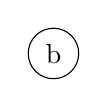
\begin{tikzpicture}\node[draw,circle] {b};\end{tikzpicture}}
\deleted{$\lambda_!\lambda^*(l_\bullet)\longrightarrow l_\bullet x$}

\deleted{$\lambda_!\lambda^*(l_\bullet)$ asphérique}
\deleted{$\unsure{Z^{(S)}}$}

(i) Si $l_\bullet$ \deleted{\unsure{réduit en degré $0$}},
\inserted{\unsure{hom} \unsure{acyclique}}, alors
$\lambda^*(l_\bullet)\deleted{\unsure{\otimes x}}\inserted{\otimes x}$
\deleted{\unsure{As}} \uline{acyclique}, pour \uline{tout $x$ [projectif]}

(ii) Si $l_\bullet$ est homotop. à $0$, alors $\lambda^*(l_\bullet)\otimes x$
acyclique pour tt $x$

(ii') $\lambda^*(\Theta_k)$ est acyclique.

(iii) $\deleted{\unsure{J\ Z}}\ \exists\ 1_M\xhookrightarrow{\alpha}J$
avec $\left\{\begin{array}{l}J\otimes x\text{ acyclique }\uline{\forall x\in M}\\
\alpha\otimes\mathrm{id}_x\text{ mono}\end{array}\right.$

\[
I\text{ asph sur }e\ \Longrightarrow\ J\deleted{\otimes}\otimes F\text{ acyclique}
\]
\[
\Longrightarrow\ \deleted{\unsure{Z^{(I)}\otimes F\longrightarrow F}}
\]
\[
\unsure{\in}\quad \unsure{\Longleftarrow}\quad
\unsure{\widetilde W_h^P(I)}\otimes F=\operatorname{Ker}(F^{(I)}\longrightarrow F)
\text{ est \deleted{asph} acyclique}
\]
\margin{donc $I\times X\mathbin{\text{---}}X$ équiv. faible pour tt. $X$.
$Z^{(I)}\times Z^{(X)}\longrightarrow Z^{(X)}$ équiv. faible \unsure{ab.}}

\uline{Lemme} Soit $I\in\operatorname{Ob}\widehat A$, asph. \deleted{sur} $e$.
Alors $\unsure{\widetilde W_h(I)}$ est \deleted{tot.} acyclique,
i.e. $\unsure{\widetilde W_h^P(I)}\otimes x$ est acyclique $\forall x$ dans $\widehat A$

a fortiori pour $x$ de la forme $Z^{(X)}$, ou $\unsure{Z^{(a)}}$
\[
\unsure{\widetilde W_h(I)}\otimes x\text{ est acyclique}
\]
\figure{\begin{tikzpicture}\draw (0,0)--(0.03,0.7)--(0.18,0.75);\end{tikzpicture}}

$J$ est $\otimes_M$-plat.

$J\otimes x$ acyclique pour $x$ projectif

$J\otimes x$ acyclique

\uline{Lemme} $J$ objet $\otimes_M$-plat. Conditions équivalentes

(i) $J\otimes_{\unsure{k}}x$ est \deleted{tot} acyclique pour tt $x$ dans $M$.

(ii) $J\otimes_{\unsure{k}}x\quad\rule{7cm}{0.3pt}\quad x$ projectif

i.e. $J$ est tot asph.

\uline{Corollaire} Car si c'est vrai

\figure{\begin{tikzpicture}\draw (0,0)--(5.8,0.55);\draw (6.2,0.62)--(13.2,0.8);\end{tikzpicture}}
\diagram{\begin{tikzcd}
l_\bullet\arrow[r] & l_\bullet\otimes\widetilde\Theta_k\arrow[l,bend left=55]
\end{tikzcd}}
\diagram{\begin{tikzcd}k\arrow[r]&\Theta_k\end{tikzcd}}
\diagram{\begin{tikzcd}l_\bullet\arrow[r,dash,shift left=2pt]\arrow[r,dash,shift right=2pt]&l'\end{tikzcd}}
\diagram{\begin{tikzcd}
l\otimes\Theta_k\arrow[r]&l'\\
l\arrow[u]&
\end{tikzcd}}
\mspage{57}
\scanpage{59}
local Ab test \unsure{category}

$l_\bullet\otimes\Theta_k$

\diagram{\begin{tikzcd}
\deleted{\unsure{Z}}\quad 1_M\arrow[r,hook]&J\arrow[r,"?"]&\lambda^*(\widetilde\Theta)
\end{tikzcd}}
\diagram{\begin{tikzcd}\lambda_!(J)\arrow[r]&\widetilde\Theta\end{tikzcd}}
\diagram{\begin{tikzcd}k^{\unsure{3|1}}\arrow[r]&k^2\end{tikzcd}}
\diagram{\begin{tikzcd}
0\arrow[r]&\widetilde\Theta_k\arrow[r]&\Theta_k\arrow[r]&k\arrow[r,dash]&0\\
&&\deleted{\unsure{J}}\quad\deleted{\unsure{k\otimes k}}&k\times k\arrow[u]\arrow[ul]&
\end{tikzcd}}

\diagram{\begin{tikzcd}
\unsure{C}\times\Delta_1\arrow[r,shift left=1pt]\arrow[r,leftarrow,shift right=1pt]&C\\
C\arrow[u,shift left=2pt]\arrow[u,shift right=2pt]&
\end{tikzcd}}
\diagram{\begin{tikzcd}
i^*(C)\times i^*(\Delta^1)\arrow[r]&i^*(C)\\
i^*(C)\arrow[u,shift left=2pt]\arrow[u,shift right=2pt]&
\end{tikzcd}}
\diagram{\begin{tikzcd}
\Theta_k\otimes l\arrow[r]&l'\\
l\arrow[u,shift left=2pt]\arrow[u,shift right=2pt]\arrow[ur,shift left=2pt]\arrow[ur,shift right=2pt]&
\end{tikzcd}}

\rotatebox{180}{\begin{minipage}{\textwidth}
\diagram{$\begin{array}{lllllllllllll}
\texttt{****A}&\texttt{END}&\texttt{JOB}&\texttt{9577}&\texttt{PLOTEDIT}&\texttt{ROOM}&\texttt{12.14.54 PM 26 AUG 82}&\texttt{R6.PR1}&\texttt{SYS JES2}&\texttt{JOB 9577}&\texttt{END}&\texttt{A****}\\
\texttt{****A}&\texttt{END}&\texttt{JOB}&\texttt{9577}&\texttt{PLOTEDIT}&\texttt{ROOM}&\texttt{12.14.54 PM 26 AUG 82}&\texttt{R6.PR1}&\texttt{SYS JES2}&\texttt{JOB 9577}&\texttt{END}&\texttt{A****}\\
\texttt{****A}&\texttt{END}&\texttt{JOB}&\texttt{9577}&\texttt{PLOTEDIT}&\texttt{ROOM}&\texttt{12.14.54 PM 26 AUG 82}&\texttt{R6.PR1}&\texttt{SYS JES2}&\texttt{JOB 9577}&\texttt{END}&\texttt{A****}\\
\texttt{****A}&\texttt{END}&\texttt{JOB}&\texttt{9577}&\texttt{PLOTEDIT}&\texttt{ROOM}&\texttt{12.14.54 PM 26 AUG 82}&\texttt{R6.PR1}&\texttt{SYS JES2}&\texttt{JOB 9577}&\texttt{END}&\texttt{A****}\\
\texttt{****A}&\texttt{END}&\texttt{JOB}&\texttt{9577}&\texttt{PLOTEDIT}&\texttt{ROOM}&\texttt{12.14.54 PM 26 AUG 82}&\texttt{R6.PR1}&\texttt{SYS JES2}&\texttt{JOB 9577}&\texttt{END}&\texttt{A****}\\
\texttt{****A}&\texttt{END}&\texttt{JOB}&\texttt{9577}&\texttt{PLOTEDIT}&\texttt{ROOM}&\texttt{12.14.54 PM 26 AUG 82}&\texttt{R6.PR1}&\texttt{SYS JES2}&\texttt{JOB 9577}&\texttt{END}&\texttt{A****}
\end{array}$}
\end{minipage}}

\diagram{\begin{tikzcd}l_\bullet\arrow[r]&U\end{tikzcd}}
\diagram{\begin{tikzcd}
\lambda^*(l_\bullet)\arrow[r]&\lambda^*(\unsure{l_\bullet}\otimes\unsure{\lambda^*}(\widetilde\Theta_k))\\
&\unsure{\lambda^*}(l_\bullet)\otimes\unsure{\lambda^*}(\widetilde\Theta_k)\arrow[u,"\unsure{\wr}"]
\end{tikzcd}}

\rotatebox{180}{\begin{minipage}{\textwidth}
\diagram{$\unsure{\begin{array}{llllllll}
\texttt{PPPPPPPPPPP}&\texttt{LL}&\texttt{OOOOOOOOOOOO}&\texttt{TTTTTTTTTTTT}&\texttt{EEEEEEEEEEEE}&\texttt{DDDDDDDDD}&\texttt{IIIIIIIIII}&\texttt{TTTTTTTTTTTT}\\
\texttt{PPPPPPPPPPPP}&\texttt{LL}&\texttt{OOOOOOOOOOOO}&\texttt{TTTTTTTTTTTT}&\texttt{EEEEEEEEEEEE}&\texttt{DDDDDDDDDD}&\texttt{IIIIIIIIII}&\texttt{TTTTTTTTTTTT}\\
\texttt{PP~~~~~~~~PP}&\texttt{LL}&\texttt{OO~~~~~~~~OO}&\texttt{~~~~~TT}&\texttt{EE}&\texttt{DD~~~~~~~DD}&\texttt{~~~~II}&\texttt{~~~~~TT}\\
\texttt{PP~~~~~~~~PP}&\texttt{LL}&\texttt{OO~~~~~~~~OO}&\texttt{~~~~~TT}&\texttt{EE}&\texttt{DD~~~~~~~~DD}&\texttt{~~~~II}&\texttt{~~~~~TT}\\
\texttt{PP~~~~~~~~PP}&\texttt{LL}&\texttt{OO~~~~~~~~OO}&\texttt{~~~~~TT}&\texttt{EE}&\texttt{DD~~~~~~~~DD}&\texttt{~~~~II}&\texttt{~~~~~TT}\\
\texttt{PPPPPPPPPPPP}&\texttt{LL}&\texttt{OO~~~~~~~~OO}&\texttt{~~~~~TT}&\texttt{EEEEEEEE}&\texttt{DD~~~~~~~~DD}&\texttt{~~~~II}&\texttt{~~~~~TT}\\
\texttt{PPPPPPPPPPP}&\texttt{LL}&\texttt{OO~~~~~~~~OO}&\texttt{~~~~~TT}&\texttt{EEEEEEEE}&\texttt{DD~~~~~~~~DD}&\texttt{~~~~II}&\texttt{~~~~~TT}\\
\texttt{PP}&\texttt{LL}&\texttt{OO~~~~~~~~OO}&\texttt{~~~~~TT}&\texttt{EE}&\texttt{DD~~~~~~~~DD}&\texttt{~~~~II}&\texttt{~~~~~TT}\\
\texttt{PP}&\texttt{LL}&\texttt{OO~~~~~~~~OO}&\texttt{~~~~~TT}&\texttt{EE}&\texttt{DD~~~~~~~~DD}&\texttt{~~~~II}&\texttt{~~~~~TT}\\
\texttt{PP}&\texttt{LL}&\texttt{OO~~~~~~~~OO}&\texttt{~~~~~TT}&\texttt{EE}&\texttt{DD~~~~~~~DD}&\texttt{~~~~II}&\texttt{~~~~~TT}\\
\texttt{PP}&\texttt{LLLLLLLLLLLL}&\texttt{OOOOOOOOOOOO}&\texttt{~~~~~TT}&\texttt{EEEEEEEEEEEE}&\texttt{DDDDDDDDDD}&\texttt{IIIIIIIIII}&\texttt{~~~~~TT}\\
\texttt{PP}&\texttt{LLLLLLLLLLLL}&\texttt{OOOOOOOOOOOO}&\texttt{~~~~~TT}&\texttt{EEEEEEEEEEEE}&\texttt{DDDDDDDDD}&\texttt{IIIIIIIIII}&\texttt{~~~~~TT}
\end{array}}$}
\end{minipage}}

\rotatebox{180}{\begin{minipage}{\textwidth}
\texttt{//*\quad PLOTEDIT9577\qquad I}
\diagram{$\unsure{\begin{array}{llll}
\texttt{~~~~~~~~00000000}&\texttt{~~~~~~~~00000000}&\texttt{~~~~~~~~00000000}&\texttt{~~~~~~~~00000000}\\
\texttt{~~~~~~0000000000}&\texttt{~~~~~~0000000000}&\texttt{~~~~~~0000000000}&\texttt{~~~~~~0000000000}\\
\texttt{~~~~00~~~~~~0000}&\texttt{~~~~00~~~~~~0000}&\texttt{~~~~00~~~~~~0000}&\texttt{~~~~00~~~~~~0000}\\
\texttt{~~~00~~~~00~00}&\texttt{~~~00~~~~00~00}&\texttt{~~~00~~~~00~00}&\texttt{~~~00~~~~00~00}\\
\texttt{~~00~~~~00~~00}&\texttt{~~00~~~~00~~00}&\texttt{~~00~~~~00~~00}&\texttt{~~00~~~~00~~00}\\
\texttt{~00~~~~00~~~00}&\texttt{~00~~~~00~~~00}&\texttt{~00~~~~00~~~00}&\texttt{~00~~~~00~~~00}\\
\texttt{00~~~~00~~~~00}&\texttt{00~~~~00~~~~00}&\texttt{00~~~~00~~~~00}&\texttt{00~~~~00~~~~00}\\
\texttt{00~~~00~~~~~00}&\texttt{00~~~00~~~~~00}&\texttt{00~~~00~~~~~00}&\texttt{00~~~00~~~~~00}\\
\texttt{0000~~~~~~~~00}&\texttt{0000~~~~~~~~00}&\texttt{0000~~~~~~~~00}&\texttt{0000~~~~~~~~00}\\
\texttt{000~~~~~~~~~00}&\texttt{000~~~~~~~~~00}&\texttt{000~~~~~~~~~00}&\texttt{000~~~~~~~~~00}\\
\texttt{0000000000}&\texttt{0000000000}&\texttt{0000000000}&\texttt{0000000000}\\
\texttt{00000000}&\texttt{00000000}&\texttt{00000000}&\texttt{00000000}
\end{array}}$}
\end{minipage}}
\mspage{58}
\scanpage{61}
\diagram{\begin{tikzcd}[column sep=large]
\underbrace{\operatorname{Hom}(X_\bullet,P_\bullet)}\otimes_k
\underbrace{\operatorname{Hom}(Y_\bullet,Q_\bullet)}
\arrow[r]&\operatorname{Hom}(X_\bullet\boxtimes Y_\bullet,P_\bullet\boxtimes Q_\bullet)\\
Z^0(\check X_\bullet\otimes P)\otimes_k Z^0(\check Y_\bullet\otimes Q_\bullet)\arrow[r]&
\deleted{\unsure{Z^0(\check X_\bullet\operatorname{Hom}}}\,
Z^{00}\bigl((\check X_\bullet\boxtimes\check Y_\bullet)\otimes(P_\bullet\boxtimes Q)\bigr)
\end{tikzcd}}

\diagram{\begin{tikzcd}[column sep=small,row sep=small]
&&&0\arrow[d]\\
&&&k\arrow[d]\\
&&k\arrow[r,dash]\arrow[d]&k\\
&k\arrow[r,dash]\arrow[d]&k&\\
k\arrow[r,dash]&k&&\\
\cdots&&&
\end{tikzcd}}
\diagram{\begin{tikzcd}[row sep=small]
0\arrow[d]\\C^0\arrow[d]\\C^1\arrow[d]\\C^{\unsure{2}}\arrow[d]\\C^3\arrow[d]\\\vdots
\end{tikzcd}}
\[
Z_n(P_\bullet)\otimes Z_m(Q_\bullet)\simeq Z_{n,m}(P_\bullet\boxtimes Q_\bullet)
\]
\diagram{\begin{tikzcd}[column sep=small]
\deleted{\unsure{\Theta}}\ L'_{n+1}\arrow[r,dash]&L'_n\arrow[r,dash]&L'_{n-1}\\
\cdots\mathbin{\text{---}}L_{n+1}\arrow[r,"\sim"']\arrow[u]&L_n\arrow[u]\arrow[ul]\arrow[r,dash]&0
\end{tikzcd}}
\[
\operatorname{Hom}(k,L)\simeq L_0
\]
\[
\operatorname{Hom}(\Theta[n],L^{\unsure{\alpha}})\simeq L_{n+1}^{\unsure{F}}
\]
\[
\operatorname{Hom}(\Theta[m],L)\simeq L_{m+1}
\]
\deleted{$\operatorname{Hom}(\Theta[n],\unsure{\boxtimes}$}
\[
\operatorname{Hom}(\Theta[n]\boxtimes\Theta[m],P_\bullet\boxtimes Q_\bullet)
\simeq(P_{\unsure{n}}\boxtimes Q_m)_{\unsure{n+1,m+1}}
\]
\[
\operatorname{Hom}(\Theta[n]\boxtimes k,P_\bullet\boxtimes Q_\bullet)
\simeq(P_\bullet\deleted{\unsure{\otimes}}\boxtimes Q_\bullet)_{n,0}
\]
\[
\operatorname{Hom}\bigl(k\boxtimes\Theta[n],P_\bullet\boxtimes Q\bigr]
\simeq[P\boxtimes Q]_{0,n}
\]
\[
\operatorname{Hom}(k\boxtimes k,P_\bullet\boxtimes Q_\bullet)
\simeq[P_\bullet\boxtimes Q_\bullet]_{0,0}
\]
\figure{\begin{tikzpicture}\draw (0,0) .. controls (5,0.6) and (11,0.8) .. (15,0.25);\end{tikzpicture}}

\diagram{\begin{tikzcd}[column sep=small,row sep=small]
&0\\
k\arrow[r,dash,"\sim"]\arrow[ur,dash]&k\arrow[u]\arrow[r,dash]\arrow[d,"\unsure{2}"']&\phantom{k}\\
k\arrow[u,"\unsure{2}"]\arrow[uur,dash]\arrow[r,"\sim"]&k\arrow[ul,dash]&
\end{tikzcd}}
$\mathrm{Ch}_\bullet(\mathrm{Ab}_k)$

$\mathrm{Ch}$
\[
\mathrm{Ch}_\bullet(P^{\unsure{\flat|h}})\simeq
(\Lambda_\bullet\otimes_{\mathbf Z}P)^{\unsure{\flat|h}}
\]
\[
\mathbf P\qquad\mathrm{Ch}_\bullet\qquad\mathrm{Ch}_\bullet
\]
\figure{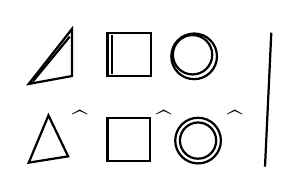
\begin{tikzpicture}[line width=0.8pt]
\draw (0,0)--(0.55,0.1)--(0.55,0.7)--cycle;
\draw (0.05,0.03)--(0.52,0.6);\draw (1,0.1)rectangle(1.55,0.65);
\draw (1.06,0.12)--(1.06,0.62);\draw (2.1,0.35)circle(0.29);
\draw (2.08,0.37)circle(0.25);
\draw (0,-1)--(0.5,-0.92)--(0.25,-0.4)--cycle;
\node at (0.65,-0.46) {$\widehat{\phantom{a}}$};
\draw (1,-0.98)rectangle(1.54,-0.43);\node at(1.72,-0.46){$\widehat{\phantom{a}}$};
\draw (2.15,-0.72)circle(0.29);\draw (2.15,-0.72)circle(0.23);
\node at(2.62,-0.46){$\widehat{\phantom{a}}$};\draw(3,-1.05)--(3.08,0.65);
\end{tikzpicture}}
$\mathrm{ch}_\bullet$
\[
\mathrm{ch}_\bullet^{\unsure{k}}\simeq\deleted{k\otimes}\mathrm{ch}_\bullet\otimes_{\mathbf Z}k
\]
\[
\mathrm{ch}_\bullet^{\unsure{\flat|h}}\simeq\mathrm{Ch}_\bullet(\mathrm{Ab})
\]
\[
\mathrm{ch}_{\bullet A}^{\deleted{\unsure{\flat}}\unsure{\sharp}}\simeq\mathrm{Ch}_\bullet(A)
\]
\[
\mathrm{ch}_\bullet\otimes\mathrm{ch}_\bullet\simeq
\text{\inserted{bi}complexe de chaînes}
\]
\[
\mathrm{ch}_{\bullet A^{\unsure{\flat}}}^{\unsure{\flat}}
\simeq\mathrm{Ch}_\bullet(A^{\unsure{\flat}})\simeq
\deleted{\unsure{A}}(\mathrm{ch}_\bullet\otimes_{\mathbf Z}A)^{\unsure{\sharp}}
\]
\margin{\figure{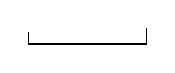
\begin{tikzpicture}\draw(0,0.15)--(0,0)--(1.5,0)--(1.5,0.2);\end{tikzpicture}}
complexes de chaînes dans $A$ qui sont homotopes à un complexe constant}
\[
\overset{n}{\bigotimes}\mathrm{ch}_\bullet=\mathrm{ch}_{(n)}
=\mathrm{ch}\deleted{\unsure{_{n,n}}}
\]
$\mathrm{Ch}_\bullet$
\[
\deleted{\unsure{\mathrm{ch}_\bullet^A\simeq}}\ \simeq\mathrm{ch}_\bullet\otimes_{\mathbf Z}A
\]
\mspage{60}
\scanpage{62}
\texttt{TRACEUR J\quad BUFFER 1020\quad BANDE 9 PISTES\quad PLUMES : 3\quad XMAX = 10100.0\quad YMAX = 70.0\quad STNB = 100.00000}

\texttt{26/ 8/ 82\qquad12 HEURES 12 MINUTES}

\texttt{JOB\qquad BANDE IBM NUMERO}

\unsure{\texttt{****************************************}}

\texttt{TRACEUR UTILISE}

\texttt{REMISE DE LA BANDE}

\texttt{DEBUT DE TRAITEMENT}

\texttt{FIN DE TRAITEMENT}

\texttt{REMISE DES GRAPH.}

\texttt{INCIDENTS SURVENUS}

\diagram{\begin{tikzcd}\widehat\Delta_{\mathrm{ab}}\arrow[r]&\mathrm{Ch}_\bullet(\mathrm{Ab})\end{tikzcd}}
$\check\Delta_{\mathrm{ab}}$

$\Phi/k_\Delta$

\diagram{$\begin{array}{llllllllllll}
\texttt{PLOT 48}&&\texttt{BLANC}&&&&&&\texttt{0}&&\texttt{0}&\\
\texttt{CNU*0399}&\texttt{GRAPHI3}&&&\texttt{JB}&\texttt{82238}&\texttt{121216}&&\texttt{0}&&\texttt{0}&\\
\texttt{GRAPHI3}&\texttt{CNU*0399}&\texttt{82238}&\texttt{M06}&\texttt{P02900500}&&\texttt{7}&\texttt{0}&\texttt{0}&&\texttt{0}&\texttt{4}\\
\texttt{CNU*0400}&\texttt{GRAPHI4}&&&\texttt{JB}&\texttt{82238}&\texttt{121217}&&\texttt{0}&&\texttt{0}&\\
\texttt{GRAPHI4}&\texttt{CNU*0400}&\texttt{82238}&\texttt{M06}&\texttt{P02900500}&&\texttt{7}&\texttt{1}&\texttt{0}&&\texttt{0}&\texttt{4}
\end{array}$}

\diagram{\begin{tikzcd}0\arrow[r]&k_\Delta\arrow[r]&\Phi\arrow[r]&K[1,\mathbf Z]\arrow[r,dash]&0\end{tikzcd}}
\[
\bigwedge^i\Phi/k\qquad\overset{i}{\bigotimes}\Phi/k
\]
\figure{\begin{tikzpicture}[scale=.8]
\draw(0,0)--(0,4.4);\draw(.55,-.65)--(.55,4.2);\draw(0,0)--(4.5,0);
\draw(.55,-.7)--(4.5,-.7);\draw(0,.55)--(1.1,.55)--(1.1,-.7);
\draw(0,1.1)--(1.1,1.1)--(1.1,.55)--(1.65,.55)--(1.65,-.7);
\draw(0,1.75)--(.55,1.75);\draw(2.2,0)--(2.2,-.7);
\draw(-.12,-.04)--(-.12,-.36)--(.33,-.36);
\node at(-.1,-.65){$0$};\draw(.18,-.68)--(.4,-.68);
\end{tikzpicture}}
\figure{\begin{tikzpicture}
\fill(0,0)circle(.035);\fill(0,.45)circle(.035);\fill(0,.72)circle(.035);\fill(0,1.05)circle(.035);
\fill(.6,1.55)circle(.035);\fill(.6,1.25)circle(.035);\fill(.6,.98)circle(.035);\fill(.6,.65)circle(.035);\fill(.6,.4)circle(.035);
\fill(0,-.55)circle(.035);\draw[->](.18,-.55)--(.6,-.55);
\end{tikzpicture}}
\[
K_{p,q}\quad p,q\geq0
\]
\[
\unsure{p+q>0}\quad\text{i.e. }(p,q)\ne0
\]
\[
p+q=n+1
\]
\[
K_{1,0}+K_{0,1}\qquad K_{0,0}=0
\]
\diagram{\begin{tikzcd}
P\arrow[r]\arrow[rr,bend left=35,"\lambda_\bullet"]&\unsure{\mathcal P}\arrow[r,shift left=1pt,"\lambda_!"]&\mathrm{Ch}_\bullet(\mathrm{Ab})\arrow[l,shift left=2pt,"\lambda^*"]
\end{tikzcd}}
\deleted{$\unsure{k}$}
\deleted{$\unsure{\lambda_!}(x)$}
\diagram{\begin{tikzcd}
l_\bullet\arrow[r]&l_\bullet\otimes\Theta\arrow[l,bend right=50]
\end{tikzcd}}
\[
x\longmapsto\operatorname{Hom}(\lambda_\bullet(x),l_\bullet)
\]
\diagram{\begin{tikzcd}
\lambda^*(l_\bullet)\arrow[r]&\lambda^*(l_\bullet\underbrace{\otimes\Theta}_{\text{Mapping cone sur }l_\bullet})\arrow[l,bend right=50]
\end{tikzcd}}
\[
\lambda^*(l_\bullet)\otimes\lambda^*(\Theta)
\]
\[
\lambda^*(\Theta[n])=C^{\unsure{n+1}}
\]
\[
\lambda^*(\mathbf Z)=C^0
\]
\diagram{\begin{tikzcd}
C^0\arrow[r]\arrow[r,bend left=30]&C^{\unsure{1}}&C^2\arrow[l]
\end{tikzcd}}
\diagram{\begin{tikzcd}[column sep=small,row sep=small]
&\vdots&&&&\\
&k\arrow[d,"\alpha"]&\unsure{k[1]}\arrow[d]&&&\\
0\arrow[r]&\Theta\deleted{\unsure{\alpha}}\arrow[r]\arrow[d,"\beta"]&\Theta[1]\arrow[r,dash]\arrow[d]&\Theta[2]\arrow[r,dash]&\cdots&\\
&k[1]\arrow[d]&\unsure{k[2]}&&&\\
&\vdots&&&&
\end{tikzcd}}
$C$
\diagram{\begin{tikzcd}[column sep=small,
execute at end picture={
\draw[decorate,decoration={brace,amplitude=3pt}]
([yshift=3pt]\tikzcdmatrixname-1-2.north west)--([yshift=3pt]\tikzcdmatrixname-1-4.north east);
\draw[decorate,decoration={brace,amplitude=3pt,mirror}]
([yshift=-4pt]\tikzcdmatrixname-1-4.south east)--([yshift=-4pt]\tikzcdmatrixname-1-6.south east);
}]
0\arrow[r,dash]&k\arrow[r]&\Theta\arrow[r]&k[1]\arrow[r]&\Theta[1]\arrow[r,dash]&k[2]\arrow[r,dash]&\Theta[2]\arrow[r,dash]&k[3]\arrow[r]&\cdots
\end{tikzcd}}
$\lambda^*(k)$
\diagram{\begin{tikzcd}[column sep=small,row sep=small]
&&0\arrow[r,dash]\arrow[d]&k\arrow[r,dash]\arrow[d]&k\arrow[r,dash]\arrow[d]&0\\
&0\arrow[r,dash]&k\arrow[r,dash]\arrow[d]&k\arrow[r,dash]\arrow[d]&0&\\
0\arrow[r,dash]&k\arrow[r,dash]&k\arrow[r]&\unsure{0}&&
\end{tikzcd}}
\mspage{61}
\scanpage{63}
\diagram{\begin{tikzcd}M\arrow[r]&P\end{tikzcd}}
\diagram{\begin{tikzcd}
M^{\unsure{\flat|h}}\arrow[r,shift left=2pt,"i_!"]\arrow[r,shift right=7pt,"i_*"']&P^{\unsure{\flat|h}}\arrow[l,"i^*"]
\end{tikzcd}}
\[
\begin{aligned}
i_*(F)(y)&=\operatorname{Hom}(y,i_*(F))\\
&=\operatorname{Hom}(i^*(y),F)
\end{aligned}
\]
\[
\delta_{M*}\lambda_{\unsure{\bullet}}^*\longrightarrow
(\lambda\boxtimes\lambda)^*\delta_{\mathrm{ch}_\bullet*}
\]
\deleted{$\unsure{\lambda}$}

\deleted{$\mathrm{ch}_\bullet$}
\diagram{\begin{tikzcd}[column sep=large,row sep=large]
\mathrm{Ch}_{\bullet\bullet}(\mathrm{Ab})\arrow[r,"(\lambda\boxtimes\lambda)^*"]\arrow[d,"\delta_{\mathrm{ch}_\bullet}^*"']&
\mathcal M\widehat\otimes\mathcal M=(M\otimes M)^{\unsure{\flat|h}}\arrow[d,"\delta_M^*"]\\
\mathrm{Ch}_\bullet(\mathrm{Ab})\arrow[r,leftrightarrow]&\mathcal M
\end{tikzcd}}
\diagram{\begin{tikzcd}M\times\mathrm{ch}_\bullet^o\arrow[r]&\mathrm{Ab}\end{tikzcd}}
\[
\Lambda(x\boxtimes y)=\lambda(x)\boxtimes\lambda y
\]
\diagram{\begin{tikzcd}M\arrow[r]&\mathrm{ch}_\bullet^{\unsure{\flat|h}}=\mathrm{Ch}_\bullet\end{tikzcd}}
\diagram{\begin{tikzcd}\mathrm{ch}_\bullet^o\arrow[r]&M^{o\unsure{\flat|h}}\end{tikzcd}}
\diagram{\begin{tikzcd}\mathbf M\boxtimes M\arrow[r]&\mathrm{Ch}_{\bullet\bullet}(\mathrm{Ab})\end{tikzcd}}
\diagram{\begin{tikzcd}\mathrm{ch}_\bullet\arrow[r]&1\arrow[r]&\mathrm{Ch}_\bullet(\mathrm{Ab}_k)\end{tikzcd}}
\deleted{\unsure{Objet final}}
\diagram{\begin{tikzcd}[column sep=large,row sep=large]
\mathrm{Ch}_\bullet(\mathrm{Ab}_k)&M\arrow[l,"\lambda_\bullet"']\\
\mathrm{Ch}_{\bullet\bullet}(\mathrm{Ab}_k)\arrow[u,"\unsure{\kappa_!^{\mathrm{ch}}}"']&M\boxtimes M\arrow[l,"\lambda_\bullet\boxtimes\lambda_\bullet"']\arrow[u,"\kappa_!^M"]\\
\mathrm{Ch}_\bullet(\mathrm{Ab}_k)\arrow[u,"\delta_{\mathrm{ch}_\bullet,!}"']\arrow[uu,bend left=55,"\mathrm{id}"]&M\arrow[l,"\lambda_\bullet"']\arrow[u,"\delta_M"]\arrow[uu,bend right=55,"\mathrm{id}"']
\end{tikzcd}}
\figure{\begin{tikzpicture}
\draw(0,0) .. controls (2,0) and (3,0.05) .. (4,0.35) .. controls (4.5,0.55) and (4.6,1.2) .. (5.4,1.3)
.. controls(6.2,1.4)and(6.4,.65)..(8,.65) .. controls(8.8,.6)and(8.8,-1.3)..(9,-3.5);
\end{tikzpicture}}
\[
\begin{aligned}
x\boxtimes y&\longmapsto\lambda_\bullet(x)\boxtimes\lambda_\bullet\unsure{[y]}\\
&\longmapsto\lambda_\bullet(x)\boxtimes\varphi(y)
\end{aligned}
\]
\[
\delta_M(\unsure{\xi})=\unsure{\xi}\otimes1\longrightarrow\lambda_\bullet(\unsure{\xi})
\]
$\lambda_\bullet$
\mspage{62}
\scanpage{64}
\rotatebox{180}{\begin{minipage}{\textwidth}
Recommandations pour la \deleted{photocopie}\inserted{xérographie} de ``Modelizing Story'' , pages 259 à 381:

1) Attention àu\deleted{x} centrage, pour ne pas couper une partie du texte

2) Faire attention aux.pages 274 et 275\inserted{*}, qui par erreur ont été frappées recto-verso (ne pas oublier donc la page 275 au verso !)

Faire une copie supplémentaire de la page 275.

3) \deleted{\unsure{Photoco}}\inserted{Faire la} copie en trois exemplaires, me renvoyer \deleted{\unsure{l'un}}\inserted{l'original} à mon do-
micile (Les Aumettes, 84570 Mormoiron), et envoyer \deleted{les} deux \deleted{autres}\inserted{copies} aux adresses suivantes:

\begin{tabular}{l}
Ronnie Brown\\
School of Mathematics\\
University College of N\unsure{g|o}rth Wales\\
Bangor, Gwynned LL 57 2 U W\\
Angleterre
\end{tabular}

et

\begin{tabular}{l}
Zoghman Mebkhout\\
68 rue du Moulin de la Pointe\\
75013 Paris
\end{tabular}

Remettre la troisième copie à Monsieur Contou-Carrère.

- Avec \unsure{mes} \unsure{remerciements|remerciement}

A \unsure{Grothendieck}

* Plus trois pages de table des matières.

PS Comme je suis absent de chez moi jusque vers le six août, il serait préférable de ne renvoyer l'original que vers le quatre ou le cinq août.
\end{minipage}}
\mspage{63}
\scanpage{65}
\diagram{\begin{tikzcd}
\mathcal M\arrow[r,shift left=2pt,"\lambda_!"]\arrow[d,equal]&\mathrm{Ch}_\bullet(\mathrm{Ab})\arrow[l,shift left=2pt,"\lambda^*"]\\
M^{\unsure{\flat|h}}&
\end{tikzcd}}
$\lambda^*($

\diagram{\begin{tikzcd}[column sep=large,row sep=large]
\mathcal M\widehat\otimes\mathcal M\arrow[r,"(\lambda\boxtimes\lambda)_!"]\arrow[d,"\delta_M^*"']&\mathrm{Ch}_{\bullet\bullet}(\mathrm{Ab})\arrow[d,"\int=\delta_{\mathrm{ch}_\bullet}^*"]\\
\mathcal M\arrow[r,"\lambda_!"']&\mathrm{Ch}_\bullet(\mathcal M)
\end{tikzcd}}
\figure{\begin{tikzpicture}\draw[->](0,0) to[bend left=25](1.1,1);\end{tikzpicture}}
\diagram{\begin{tikzcd}
\mathrm{ch}_\bullet(\mathrm{Ab})^{\unsure{\flat|h}}\simeq\mathrm{Ch}_\bullet(\mathrm{Ab})&\mathrm{Ch}_{\bullet\bullet}^{\unsure{a}}(\mathrm{Ab})\arrow[l]
\end{tikzcd}}
\diagram{\begin{tikzcd}
\deleted{\unsure{C}}\ \mathrm{ch}_\bullet(\mathrm{Ab})\arrow[r]&\mathrm{ch}_{\bullet\bullet}(\mathrm{Ab})\quad??
\end{tikzcd}}
\figure{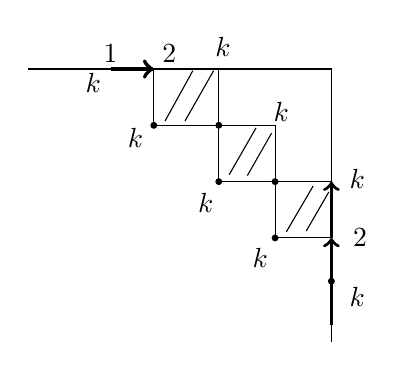
\begin{tikzpicture}[scale=1.1]
\draw(-1.2,2.7)--(2.3,2.7)--(2.3,-.45);
\draw[line width=1.5pt,->](-.25,2.7)--(.25,2.7);
\draw(.25,2.7)--(.25,2.05)--(1,2.05)--(1,1.4)--(1.65,1.4)--(1.65,.75)--(2.3,.75);
\draw(1,2.7)--(1,2.05)--(1.65,2.05)--(1.65,1.4)--(2.3,1.4);
\draw[line width=1.2pt,->](2.3,-.25)--(2.3,.75);
\draw[line width=1.2pt,->](2.3,.75)--(2.3,1.4);
\foreach \x/\y in {.25/2.05,1/2.05,1/1.4,1.65/1.4,1.65/.75,2.3/.25}{\fill(\x,\y)circle(.04);}
\draw(.38,2.1)--(.7,2.68);\draw(.61,2.1)--(.94,2.68);
\draw(1.12,1.48)--(1.43,2.02);\draw(1.33,1.47)--(1.61,1.96);
\draw(1.78,.82)--(2.09,1.35);\draw(2.01,.83)--(2.27,1.28);
\node at(-.25,2.88){$1$};\node at(.43,2.88){$2$};\node at(1.05,2.96){$k$};
\node at(-.45,2.54){$k$};\node at(.04,1.9){$k$};\node at(1.72,2.2){$k$};
\node at(.85,1.16){$k$};\node at(2.6,1.43){$k$};\node at(1.48,.52){$k$};
\node at(2.63,.75){$2$};\node at(2.6,.07){$k$};
\end{tikzpicture}}
\figure{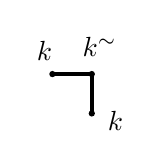
\begin{tikzpicture}[line width=1.3pt]
\draw(0,.5)--(.5,.5)--(.5,0);\fill(0,.5)circle(.04);\fill(.5,.5)circle(.04);\fill(.5,0)circle(.04);
\node at(-.1,.8){$k$};\node at(.6,.85){$k^\sim$};\node at(.8,-.1){$k$};
\end{tikzpicture}}
\diagram{\begin{tikzcd}[column sep=small]
L_{\unsure{i+1}}\arrow[r,dash]&L_i\arrow[r,dash]&L_{i-1}\\
\mathbin{\text{---}}k\arrow[r,dash]\arrow[u]&k\arrow[r,dash]\arrow[u]&0
\end{tikzcd}}
\deleted{$\operatorname{Hom}($}
\[
\operatorname{Hom}(\underbrace{L_\bullet}_{\in\mathrm{ch}_\bullet(\mathrm{Ab})},\int M_{\bullet\bullet})
\simeq\operatorname{Hom}(\underbrace{\delta(L_\bullet)}_{\in\mathrm{ch}_{\bullet\bullet}(\mathrm{Ab})\,?},M_{\bullet\bullet})
\]
\figure{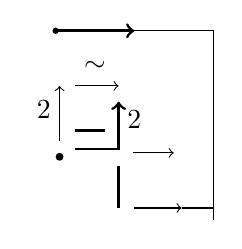
\begin{tikzpicture}
\draw[->,line width=1pt](0,1.9)--(1,1.9);\draw(1,1.9)--(2,1.9)--(2,-.5);
\fill(0,1.9)circle(.04);\fill(.05,.3)circle(.05);
\draw[->](.05,.5)--(.05,1.2);\node at(-.15,.9){$2$};
\draw[->](.25,1.2)--(.8,1.2);\node at(.5,1.45){$\sim$};
\draw[->,line width=1pt](.25,.4)--(.8,.4)--(.8,1);\node at(1,.77){$2$};
\draw[line width=1.2pt](.25,.63)--(.63,.63);\draw[->](.98,.35)--(1.5,.35);
\draw[line width=1pt](.8,.18)--(.8,-.35);\draw[->](1,-.35)--(1.6,-.35);\draw(1.6,-.35)--(2,-.35);
\end{tikzpicture}}
\[
L_\bullet=a
\]
\deleted{$\unsure{\delta L_\bullet}$}
\deleted{$\operatorname{Hom}(a,M_{0,0})=$}
\deleted{$M_{0,1}\unsure{+}M_{1,0}$}

\diagram{\begin{tikzcd}
\lambda_!(a\otimes y)\arrow[r,"\deleted{\unsure{asph}}\inserted{\text{qu.iso}}"]&\lambda_!(a)\otimes\lambda_!(y)
\end{tikzcd}}
\diagram{\begin{tikzcd}
\lambda^*(\xi\otimes\eta)&\lambda^*(\xi)\otimes\arrow[l,"\unsure{\sim}"]
\end{tikzcd}}
\diagram{\begin{tikzcd}[column sep=large]
\lambda^*(L_\bullet\otimes M_\bullet)\arrow[r,leftrightarrow,"\substack{W_M\ ?\\\deleted{\text{qu.iso}}}"]&\lambda^*(L_\bullet)\otimes\lambda^*(M)
\end{tikzcd}}
\diagram{\begin{tikzcd}
M\otimes M\arrow[r,"\lambda\boxtimes\lambda"]&\mathrm{Ch}_{\bullet\bullet}(\mathrm{Ab})\\
M\arrow[u,"\delta_M"]\arrow[r,"\lambda"']&\mathrm{Ch}_\bullet(\mathrm{Ab})\arrow[u,"\delta"']
\end{tikzcd}}
\diagram{\begin{tikzcd}[column sep=large,row sep=large]
L_\bullet\otimes M_\bullet\quad\deleted{\unsure{M\otimes}}&
\lambda_!(\lambda^*(L_\bullet)\otimes\lambda^*(M))\arrow[l,"\text{qu.iso ?}"']\arrow[d,"\text{qu.iso}\quad\mathbf{EZ}"]\\
&\lambda_!(\lambda^*(L_\bullet))\otimes\lambda_!(\lambda^*(M))\arrow[ul]
\end{tikzcd}}
\[
M\otimes\mathbf M
\]
$\lambda^*$
\diagram{\begin{tikzcd}
P=M\otimes M\\M\arrow[u]
\end{tikzcd}}
$\operatorname{Hom}(x\boxtimes y,z)$
\diagram{\begin{tikzcd}(M\otimes M)^{\unsure{\flat|h}}\arrow[d]&\\M^{\unsure{\flat|h}}&\end{tikzcd}}
\diagram{\begin{tikzcd}\mathbf M\arrow[r]&P\end{tikzcd}}
\diagram{\begin{tikzcd}
M^{\unsure{\flat|h}}\arrow[r,shift left=2pt,"i_!"]\arrow[r,dash,shift right=7pt,"i_*"']&P^{\unsure{\flat|h}}\arrow[l,"\unsure{i^*}"]
\end{tikzcd}}
\mspage{64}
\scanpage{66}
\uline{Lemme.} $\mathcal M$ abelian \inserted{$k$-ab} cat. with \deleted{suff} $\varprojlim$ and suff.
many injectives and projectives. Assume moreover projectives are $k$-flat, \uline{or} injectives $k$-coflat. Then
for $F\in\widehat A_{\mathcal M}$, \deleted{we have} and $a$ projective in $\mathcal M$, we get
\[
\deleted{\unsure{k}}\quad u_a(RH^\bullet(A,F))\simeq RH^\bullet(A,u_a\circ F).
\]
where
\[
u_a:\mathcal M\longrightarrow\mathrm{Ab}_k:\quad x\mathbin{\text{---}}\operatorname{Hom}(a,x)
\]
\inserted{The functor $u_a$ is exact}

\uline{Proof} If $a$ is $k$-flat, then $u_a$ transforms injectives into injectives, and we get
\[
u_a\circ R\Gamma_{A,\mathcal M}\simeq
R(\underbrace{u_a\circ\Gamma_{A,\mathcal M}}_{\Gamma_{A,\mathrm{Ab}_k}\circ u_a})
\qquad\mathrm{OK}
\]
If injectives are coflat, the same holds

\[
\underbrace{\operatorname{Hom}(\underset{\mathrm{proj}}a,\deleted{\unsure{\mathbf Z}}\underset{\mathrm{inj}}x)}_{\text{inj ?}}
\]
\diagram{\begin{tikzcd}[column sep=large]
&\operatorname{Hom}_k(\unsure{\xi},\operatorname{Hom}(a,x))\arrow[dl,equal]\arrow[dr,equal]&\\
\operatorname{Hom}(\unsure{\xi}\otimes_k a,x)&&\operatorname{Hom}(a,\operatorname{Hom}_k(\unsure{\xi},x))
\end{tikzcd}}

$\Rightarrow$ Conditions équiv. sur $\mathcal M$ (:

a) les projectifs sont plats

b) les injectifs sont coplats

c) Si $a$ proj, $b$ injectif, alors $\operatorname{Hom}(a,b)$ est injectif dans $\mathrm{Ab}_k$
\mspage{65}
\scanpage{67}
\uline{Problèmes ouverts en théorie des Intersections.}

\uline{A. Grothendieck.}

\uline{Exposé $\overline{\underline{\mathrm{XIV}}}$}
\figure{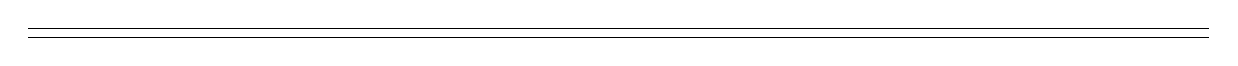
\begin{tikzpicture}\draw(0,0)--(15,0);\draw(0,.12)--(15,.12);\end{tikzpicture}}

\uline{Corrections à Faire après tirage}

\diagram{$\begin{array}{llll}
\text{p 14 -}&\text{ligne 59 -}&\text{est non nulle}&\text{(refaire NON)}\\[6pt]
\text{p 15 -}&\text{ligne 59 -}&\psi^3.&\text{(refaire }\psi\text{)}\\[6pt]
\text{p 2 -}&\text{ligne 17 -}&\overset{i}{\otimes}{}^L L.&\text{(refaire }\otimes\text{)}\\[6pt]
\text{p 19 -}&\text{ligne 3 -}&\text{7. clesses}&\text{(au lieu de cl\uuline{a}sses)}\\[6pt]
\text{p 17 -}&\text{ligne 12 -}&\text{\unsure{flêches|flâches}}&\text{(au lieu de fléches)}
\end{array}$}

\[
x\longmapsto\operatorname{Hom}(x,\unsure{\xi})\qquad\unsure{\xi}\text{ injectif}
\]
\diagram{\begin{tikzcd}
B^o\arrow[r,"F"]&\mathrm{Ab}_k\arrow[r,"\deleted{\unsure{*}}v"]&\mathrm{Ab}_k^o
\end{tikzcd}}
\diagram{\begin{tikzcd}B^o\arrow[r,dash]&\mathrm{Ab}_k\end{tikzcd}}
injectifs $\Longrightarrow$ injectifs de $\mathrm{Ab}_k^o$

i.e. des \uline{projectifs} de $\mathrm{Ab}_k$

\diagram{\begin{tikzcd}B^o\arrow[r]&\mathrm{Ab}\end{tikzcd}}
\deleted{$\unsure{\mathrm{Ab}_k}$}
\diagram{\begin{tikzcd}\mathcal M\arrow[r,"u"]&\mathcal M'\end{tikzcd}}
$u$ \uline{exact}, transforme injectifs en injectifs

\deleted{$\unsure{H^i}\quad C(F$}
$C^i$
\deleted{$\unsure{\mathrm{Ab}_k}$}
\[
\deleted{\unsure{t}}\ v(R\Gamma_{\unsure{\mathrm{Ab}_k}}(B,F))
\overset{?}{\simeq}R\Gamma(B,v\circ F)
\bigl(\simeq LH_\bullet(A^o,(v\circ F)^o)\bigr)
\]
$\Gamma(C^i)$
\figure{\begin{tikzpicture}
\draw(0,.1)..controls(2,0)and(3,-.2)..(4,-.1)..controls(4.8,0)and(4.2,.8)..(4.9,.95)..controls(6,1.2)and(8,1.3)..(9,1.15);
\end{tikzpicture}}
\[
LH_0(A,\int F)\mathbin{\text{---}}LH_\bullet(B,F)
\]
\[
F\in\widehat B_{\mathcal M}
\]
\diagram{\begin{tikzcd}\mathcal M\arrow[r]&\mathrm{Ab}_k\end{tikzcd}}
commute aux $\varinjlim$ et transforme projectifs en projectifs

\uline{ex.} $\mathcal M=M^{\unsure{\flat|h}}$,
\diagram{\begin{tikzcd}\mathrm{Ab}_k^o\arrow[r,"\text{contre}"]&\mathrm{Ab}_k\end{tikzcd}}
\mspage{66}
\scanpage{68}
\diagram{\begin{tikzcd}A\arrow[r,"f"]&B\end{tikzcd}}

$f$ $\unsure{W_h|W_k}$-asph, i.e. $\forall b\in\operatorname{Ob}B$, on a
\[
-\qquad \underbrace{A_{/b}}_{\displaystyle\substack{\Vert\\ A/f^*(b)}}\longrightarrow B_{/b}
\qquad\text{une }\unsure{W_h|W_k}\text{-équiv.}
\]
i.e.
\[
LH_\bullet\left(A,\underbrace{\mathbb Z^{(f^*b)}}_{f^*(\mathbb Z^{(b)})}\right)
\longrightarrow LH_\bullet(B,\mathbb Z^{(b)})\qquad\text{iso}
\]
\figure{\begin{tikzpicture}\draw(0,0)..controls(5,.1)and(10,.6)..(14,.8);\end{tikzpicture}}
\[
LH_\bullet(A,f^*F)\xrightarrow{\simeq}LH_\bullet(B,F).
\]
\[
\forall F\in\widehat B_{\mathcal M}\qquad
\mathcal M\ \inserted{\text{$k$-add avec}}\ \text{\uline{assez de projectifs}}
\]
\[
LH^\bullet(B^o,\unsure{G|F})\overset{\simeq}{\mathbin{\text{---}}}LH^\bullet(A^o,f^*G)
\qquad\text{si }G\in\widehat{B^o}_{\mathcal N},\quad\mathcal N\text{ assez d'injectifs}
\]
\diagram{\begin{tikzcd}B\arrow[r]&\mathbf M\end{tikzcd}}

$W_k$-asph\qquad $W_k$-coasph.

\[
x\longmapsto\operatorname{Hom}(a,x)\qquad\mathcal M\longrightarrow\mathrm{Ab}_k
\]
transforme injectifs en \unsure{itou} ?
\[
\operatorname{Hom}_{\mathrm{Ab}_k}(\xi,\operatorname{Hom}(a,\unsure{a|x}))
\simeq\operatorname{Hom}_k(a\otimes_k\xi,\unsure{a|x})
\]
OK si $a$ est $k$-\uline{plat} et \uline{projectif}
\mspage{67}
\scanpage{69}
Soit cat. \inserted{$k$-}abélienne $\mathcal M$
\[
\left(\begin{array}{l}
\text{avec }\varprojlim\\
\text{\uline{assez de projectifs $k$-plats}}\\
\text{assez d'injectifs.}
\end{array}\right.
\]
Alors si $f:A\mathbin{\text{---}}B$ est $k$-coasphérique, alors
\[
\unsure{LH^\bullet|LH_\bullet}(B,F)\overset{\simeq}{\mathbin{\text{---}}}LH_\bullet(A,f^*F)
\qquad\forall F\in\widehat B_{\mathcal M}
\]

\deleted{$\operatorname{Hom}(a,$}
\[
\xi\longrightarrow a\otimes_k\xi\qquad\text{transforme mono en mono.}
\]
\margin{$)$}
\[
\xi\mathbin{\text{---}}\operatorname{Hom}(\xi,a)\qquad\text{transforme mono en épi}
\]
\diagram{\begin{tikzcd}
LH_\bullet(A,F)\\
\widehat A_{\mathcal N}\arrow[u]
\end{tikzcd}}
\[
\mathbf{Ab}_k^{\deleted{\unsure{o}}}\qquad
\deleted{\text{\unsure{assez}}}\ \varinjlim
\]
assez de proj

assez d'inj. $k$-co\unsure{plats} ?

OK

\deleted{$\varinjlim$}
\figure{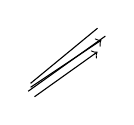
\begin{tikzpicture}
\draw[->](0,0)--(.9,.6);\draw[->](.05,-.12)--(.85,.45);
\draw(0,.05)--(.85,.75);\draw(-.03,-.05)--(.95,.65);
\end{tikzpicture}}
\[
\mathbb Q\qquad\mathbb Q_p/\mathbb Z_p
\]
$\mathrm{Ab}$\hfill$\mathbf{Ab}_k^o$
\[
x\longrightarrow\operatorname{Hom}(x,I)
\]
\diagram{\begin{tikzcd}
B\arrow[r]&\mathrm{Ab}_k\arrow[r]&\mathrm{Ab}_k^o
\end{tikzcd}}
\[
\operatorname{Hom}(J,I)\qquad\text{objet injectif de}
\]
$\mathrm{Ab}_k^o$ i.e. proj.\par
en $\mathrm{Ab}_k$
\mspage{68}
\scanpage{70}
\diagram{\begin{tikzcd}
RH^\bullet(\unsure{B|A},F)\arrow[dd]\\
\widehat B_{\mathcal M}\arrow[u]\\
RH^\bullet(A,f^*F)
\end{tikzcd}}
\[
\left[\begin{array}{l}
\mathcal M\\
\text{cat. abélienne}\\
\text{stable par }\varprojlim\\
\text{assez d'injectifs}\\
\text{\uline{assez} de proj.}
\end{array}\right.
\]
\[
R\operatorname{Hom}^{\bullet}(a,\qquad\qquad u(\Gamma(C^\bullet))
\]
$C^i$

\deleted{$\unsure{\mathrm{Ab}}$}
\diagram{\begin{tikzcd}
\widehat B_{\mathcal M}\arrow[r,"\Gamma_{\mathcal M}"]\arrow[dr]&\mathcal M\arrow[r,"{\operatorname{Hom}(a,-)}"]&\mathrm{Ab}_k\\
&\widehat B_k\arrow[ur,"\Gamma_k"']&
\end{tikzcd}}
\[
R\operatorname{Hom}(a,R\Gamma(B,F))\overset{?}{\simeq}R\Phi(F)
\]
si $\Gamma$ transforme injectifs en injectifs

\deleted{$R\operatorname{Hom}^{\bullet}(L_\bullet,F^\bullet)$}

$\operatorname{Ext}^i(a,$

\deleted{$R\Gamma$}
\[
u\bigl(\operatorname{Hom}(L_\bullet,F^\bullet)\bigr)
\]
\diagram{\begin{tikzcd}B^o\arrow[r]&\mathcal M\end{tikzcd}}
\[
R\Gamma_k\circ R\operatorname{Hom}^{\bullet}(a,F)
\]
$F^\bullet$
\diagram{$\begin{array}{l|l}
\text{Assez de proj.}&\text{proj plats}\\
\text{assez d'inj}&\text{inj. coplats}
\end{array}$}

$u(C^\bullet)$

\diagram{\begin{tikzcd}
\widehat B_{\mathcal M}\arrow[r,"\Gamma_{\mathcal M}"]&\mathcal M\arrow[r,"u\ \text{exact}"]&\mathcal M'
\end{tikzcd}}
\mspage{69}
\scanpage{71}
\[
u\bigl(\underbrace{R\Gamma_{\mathcal M}(F)}\bigr)\overset{?}{\simeq}R\Gamma_{\mathcal M'}(u(F))
\]
\[
u\bigl(\Gamma_{\mathcal M}(C^\bullet(F))\bigr)
\]
\[
\Gamma_{\mathcal M'}u\left(\underbrace{C^\bullet(F)}_{\substack{\deleted{u(C^i)}\\\text{résolution de}\\u(F)}}\right)
\]
est elle $\Gamma_{\mathcal M'}$-acyclique ?
\[
C\text{ injectif dans }\deleted{\mathrm{Ab}}\ \widehat B_{\mathcal M}
\Longrightarrow u(F)\text{ injectif dans }\widehat B_{\mathcal M'},
\]
\deleted{$u(C)$}
\[
u\bigl(\underbrace{\operatorname{Hom}^{\bullet\bullet}_k(L_\bullet,F^\bullet)}\bigr)
\simeq\operatorname{Hom}^{\bullet\bullet}_k(L_\bullet,u(F^\bullet)))
\]
\[
Ru\bigl(R\operatorname{Hom}(L_\bullet,F)\bigr)
\]
\diagram{$\mathcal M\left\{\begin{array}{ll|l}
\text{Sufficiently \uline{many}}&\text{inj.}&\text{injectives are coflat}\\
&\text{projectives}&\text{\uline{or} projectives are}\\
&&\text{flat}\\
\varprojlim\ \text{exist}&&
\end{array}\right.$}

\deleted{Alors}\quad\uline{Then}\qquad if $f:A\mathbin{\text{---}}B$ is coasph,

$F\in\widehat B_{\mathcal M}$, then
\margin{\deleted{$\unsure{A}$}}
\[
RH^\bullet(A,f^*F)\mathbin{\text{---}}RH^\bullet(B,F)
\]
We apply $\operatorname{Hom}(a,-)$ to both members,
with $a$ projective in $\mathcal M$

\deleted{\unsure{then}} let $F^a\in\widehat B_k$ deduced from $F$ :
$(b\longmapsto\operatorname{Hom}(a,F(b)))$

then\qquad $f^*(F^a)=(f^*F)^a$
\mspage{70}
\scanpage{72}
\diagram{\begin{tikzcd}
A\arrow[r]&M_{as}\arrow[r,phantom,"\subset"]\arrow[drr,bend right=18]&M\arrow[r,"\kappa"]&\mathrm{Ab}_k\\
&&&\mathrm{ab}_k\arrow[u]
\end{tikzcd}}
\[
\widehat A/X\simeq\widehat{(A_{/X})}
\]

\rotatebox{90}{\begin{minipage}{18cm}
\diagram{$\begin{array}{rlll}
&\texttt{OOOOOOOOOOOO}&\texttt{NN\ \ \ \ \ \ \ \ NN}&\texttt{TTTTTTTTTTTT}\\
\texttt{D}\ \ &\texttt{OOOOOOOOOOOO}&\texttt{NNN\ \ \ \ \ \ \ NN}&\texttt{TTTTTTTTTTTT}\\
\texttt{DD}\ &\texttt{OO\ \ \ \ \ \ \ \ OO}&\texttt{NNNN\ \ \ \ \ \ NN}&\texttt{\ \ \ \ \ TT}\\
\texttt{DD}&\texttt{OO\ \ \ \ \ \ \ \ OO}&\texttt{NN\ NN\ \ \ \ \ NN}&\texttt{\ \ \ \ \ TT}\\
\texttt{DD}&\texttt{OO\ \ \ \ \ \ \ \ OO}&\texttt{NN\ \ NN\ \ \ \ NN}&\texttt{\ \ \ \ \ TT}\\
\texttt{DD}&\texttt{OO\ \ \ \ \ \ \ \ OO}&\texttt{NN\ \ \ NN\ \ \ NN}&\texttt{\ \ \ \ \ TT}\\
\texttt{DD}&\texttt{OO\ \ \ \ \ \ \ \ OO}&\texttt{NN\ \ \ \ NN\ \ NN}&\texttt{\ \ \ \ \ TT}\\
\texttt{DD}&\texttt{OO\ \ \ \ \ \ \ \ OO}&\texttt{NN\ \ \ \ \ NN\ NN}&\texttt{\ \ \ \ \ TT}\\
\texttt{DD}&\texttt{OO\ \ \ \ \ \ \ \ OO}&\texttt{NN\ \ \ \ \ \ NNNN}&\texttt{\ \ \ \ \ TT}\\
\texttt{DD}\ &\texttt{OO\ \ \ \ \ \ \ \ OO}&\texttt{NN\ \ \ \ \ \ \ NNN}&\texttt{\ \ \ \ \ TT}\\
\texttt{D}\ \ &\texttt{OOOOOOOOOOOO}&\texttt{NN\ \ \ \ \ \ \ \ NN}&\texttt{\ \ \ \ \ TT}\\
&\texttt{OOOOOOOOOOOO}&\texttt{NN\ \ \ \ \ \ \ \ \ N}&\texttt{\ \ \ \ \ TT}
\end{array}$}
\begin{tabular}{l}
\texttt{.49.07 PM 19 MAY 82 R6.PR1 SYS JES2 JOB 1282 START A****}\\
\texttt{.49.07 PM 19 MAY 82 R6.PR1 SYS JES2 JOB 1282 START A****}\\
\texttt{.49.07 PM 19 MAY 82 R6.PR1 SYS JES2 JOB 1282 START A****}\\
\texttt{.49.07 PM 19 MAY 82 R6.PR1 SYS JES2 JOB 1282 START A****}\\
\texttt{.49.07 PM 19 MAY 82 R6.PR1 SYS JES2 JOB 1282 START A****}\\
\texttt{.49.07 PM 19 MAY 82 R6.PR1 SYS JES2 JOB 1282 START A****}
\end{tabular}
\end{minipage}}

\diagram{\begin{tikzcd}A\arrow[r]&B\end{tikzcd}}
\diagram{\begin{tikzcd}\mathrm{add}\,A\arrow[r]&\mathrm{add}\,B\end{tikzcd}}
\diagram{\begin{tikzcd}\widehat A_{ab}&\widehat B_{ab}\arrow[l]\end{tikzcd}}
\[
f^*(F)\qquad F\qquad\unsure{f_!|f^!}\quad f^*
\]
$H$
\[
\mathbb Z^{f^*(b)},\qquad\mathbb Z^{(b)}
\]
\figure{\begin{tikzpicture}\draw(0,0)--(8,0);\end{tikzpicture}}
$W_k$-asphérique
\diagram{\begin{tikzcd}A_{/f^*(b)}\arrow[r]&\unsure{B_{/b}'|B_{/b},}\end{tikzcd}}
\mspage{71}
\scanpage{73}
\deleted{$\unsure{\mathcal M|\mathrm{Ab}}$}
\deleted{$\unsure{y\longmapsto}\kappa_{\unsure{N|M}}^*\kappa_{M!}$}
\diagram{\begin{tikzcd}
\mathcal M\arrow[r,shift left=2,"f_!"]&{}\arrow[l,shift left=2,"{f^*(\xi)=1_M\otimes\xi}"]
\end{tikzcd}}
\diagram{\begin{tikzcd}{}\arrow[r,"{f_*(-)=\operatorname{Hom}(1_M,-)}"']&{}\end{tikzcd}}
\[
\alpha_\xi\simeq\alpha\otimes\xi
\]
\diagram{\begin{tikzcd}
{}\arrow[r]&f_!f^*\xi\arrow[r,"\simeq"]&f_!(1_M)\otimes\xi\arrow[r,"\alpha_\xi"]&\xi
\end{tikzcd}}
\diagram{\begin{tikzcd}f_!(1_M)\arrow[r]&k\end{tikzcd}}
\[
y\xrightarrow{\varepsilon_y}f^*f_!y\quad\in W_{\mathcal M}^{!}\ ?
\]
\diagram{\begin{tikzcd}
f_!y\arrow[r,"{f_!(\varepsilon_y)}","\text{iso ?}"']\arrow[rr,bend right=24,"\simeq"']&
f_!f^*\underbrace{f_!(y)}\arrow[r,"{\alpha_{f_!(y)}}"]&f_!y
\end{tikzcd}}

\rotatebox{90}{\begin{minipage}{15cm}
\[
x\xrightarrow[\deleted{\otimes}]{}x\otimes X\otimes X^\vee
\]
\[
f^!\unsure{f_*|f_!}z\longrightarrow z
\]
$\mathrm{Ab}$
\deleted{$X$}
\unsure{dans}
\[
\operatorname{Hom}(\qquad X\otimes\xi
\]
\figure{\begin{tikzpicture}
\draw(0,0)..controls(.2,.2)and(.3,-.1)..(.5,.05)..controls(.8,.2)and(1,.05)..(1.5,.1);
\end{tikzpicture}}
\deleted{$\unsure{\mathrm{Ab}}$}
\deleted{$\unsure{X}$}
\[
(\unsure{x},\quad x\otimes X^\vee,
\]
\[
x\longmapsto x\otimes X^\vee
\]
\end{minipage}}

\diagram{$\begin{array}{llll}
\texttt{PPPPPPPPPPP}&\texttt{RRRRRRRRRRR}&\texttt{EEEEEEEEEEEE}&\texttt{DDDDDDDD}\unsure{\texttt{D}}\\
\texttt{PPPPPPPPPPPP}&\texttt{RRRRRRRRRRRR}&\unsure{\texttt{EEEEEEEEEEEE}}&\texttt{DDDDDDDD}\unsure{\texttt{D}}\\
\texttt{PP\ \ \ \ \ \ \ \ PP}&\texttt{RR\ \ \ \ \ \ \ \ RR}&\texttt{EE}&\texttt{DD}\\
\texttt{PP\ \ \ \ \ \ \ \ PP}&\texttt{RR\ \ \ \ \ \ \ \ RR}&\texttt{EE}&\texttt{DD}\\
\texttt{PP\ \ \ \ \ \ \ \ PP}&\texttt{RR\ \ \ \ \ \ \ \ RR}&\texttt{EE}&\texttt{DD}\\
\unsure{\texttt{PPPPPPPPPPPP}}&\texttt{RRRRRRRRRRRR}&\texttt{EEEEEEEE}&\texttt{DD}\\
\unsure{\texttt{PPPPPPPPPPP}}&\texttt{RRRRRRRRRRR}&\texttt{EEEEEEEE}&\texttt{DD}\\
\texttt{PP}&\texttt{RR\ \ \ \ RR}&\texttt{EE}&\texttt{DD}\\
\texttt{PP}&\texttt{RR\ \ \ \ \ RR}&\texttt{EE}&\texttt{DD}\\
\texttt{PP}&\texttt{RR\ \ \ \ \ \ RR}&\texttt{EE}&\texttt{DD}\\
\texttt{PP}&\texttt{RR\ \ \ \ \ \ \ RR}&\texttt{EEEEEEEEEEEE}&\texttt{DDDDDDDD}\unsure{\texttt{D}}\\
\texttt{PP}&\texttt{RR\ \ \ \ \ \ \ \ RR}&\texttt{EEEEEEEEEEEE}&\texttt{DDDDDDDD}\unsure{\texttt{D}}
\end{array}$}
\begin{tabular}{l}
\texttt{****A START JOB 1282 PREDONT - CRAY OUTPUT - ROOM }\unsure{6|A}\\
\texttt{****A START JOB 1282 PREDONT - CRAY OUTPUT - ROOM }\unsure{6|A}\\
\texttt{****A START JOB 1282 PREDONT - CRAY OUTPUT - ROOM }\unsure{6|A}\\
\texttt{****A START JOB 1282 PREDONT - CRAY OUTPUT - ROOM }\unsure{6|A}\\
\texttt{****A START JOB 1282 PREDONT - CRAY OUTPUT - ROOM }\unsure{6|A}\\
\texttt{****A START JOB 1282 PREDONT - CRAY OUTPUT - ROOM }\unsure{6|A}
\end{tabular}

\texttt{DERNIERE MISE A JOUR DE JOURNAL: 17-05-82}

\rotatebox{90}{\begin{minipage}{17cm}
\[
f^*\xi\longrightarrow\kappa_M^*(\xi)
\]
\figure{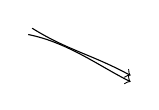
\begin{tikzpicture}
\draw[->](0,.6)..controls(.5,.5)and(.9,.2)..(1.3,0);
\draw[->](.05,.68)..controls(.5,.4)and(.8,.35)..(1.3,.08);
\end{tikzpicture}}
\deleted{$f_!f^*y\longrightarrow f_!$}
\[
\kappa_{M!}f^*y\longrightarrow\kappa_{N!}(y)
\]
\[
y\longrightarrow1_M\otimes\kappa_!(y)\qquad\text{\uline{épi}}\quad??
\]
\[
0\longrightarrow\unsure{y^\flat|y^b}\longrightarrow y\longrightarrow
\overset{=1_M\otimes\kappa_!y}{\kappa^*\kappa_!y}\longrightarrow0
\]
\[
0\mathbin{\text{---}}f^*(\unsure{y^\flat|y^b})\longrightarrow f^*(y)
\mathbin{\text{---}}f^*\kappa^*\kappa_!y
\]
\[
\operatorname{Hom}_k(\kappa_!y,\operatorname{Hom}(1_M,z))
\mathbin{\text{---}}\operatorname{Hom}(y,z)
\]
\[
\operatorname{Hom}(y,1_M\otimes\operatorname{Hom}(1_M,z))
\]
\[
1_M\otimes_k\operatorname{Hom}(1_M,z)\xrightarrow[\text{mono}]{}z
\]
\end{minipage}}
\mspage{72}
\scanpage{74}
\diagram{\begin{tikzcd}M\arrow[r]&\mathrm{ab}_k\end{tikzcd}}
$M\otimes N$
\diagram{\begin{tikzcd}X\arrow[r]&M\\X\arrow[r]&N\end{tikzcd}}
\diagram{\begin{tikzcd}
&&M\\
X\deleted{\otimes}X\arrow[r]&M\otimes N\arrow[ur]\arrow[dr]&\\
\mathbf X\arrow[u]&&N
\end{tikzcd}}

$M^{\unsure{\flat|b}}$
\[
L\kappa_M(F)=
\]
\diagram{\begin{tikzcd}\underline M\arrow[r]&M^{\unsure{\flat|b}}\end{tikzcd}}
\deleted{$\longleftrightarrow$}
\diagram{\begin{tikzcd}\unsure{1|e}_{A/x}\arrow[r]&x\end{tikzcd}}
\diagram{\begin{tikzcd}A_{/x}\arrow[r]&A\end{tikzcd}}
\[
\deleted{\unsure{e}}\ 1_{\mathrm{Add}(M_{/x})}\longrightarrow k^{(x)}
\]
\[
M^{\unsure{\flat|b}}=\mathcal M\ni F
\]
\diagram{\begin{tikzcd}N\arrow[r,"f"]&\underline M\end{tikzcd}}
a) $f_!$ exact (à g.)

b) \deleted{$f_!(1_N)=F$}\inserted{$1_N$ projectif}

c) $f_!(1_N)=F$

\fbox{\begin{minipage}{8cm}
a) $f_!$ exact ; $\unsure{f_*}$

b) $1_N\in N$

c) $f_!(1_N)=a$
\end{minipage}}
\margin{fidèle,
$\operatorname{Hom}\mathbin{\text{---}}\operatorname{Hom}$\par
\unsure{unité inj.}}
\diagram{\begin{tikzcd}a\arrow[r,bend right=18]&\text{obj. \deleted{projectif} de \inserted{en $M$}}\end{tikzcd}}
\[
f_!f^*a\mathbin{\text{---}}
\]
$\mathbb Z^{(a)}$

$\underline M^{\unsure{\flat|b}}\qquad F$
\[
N=\{F\in\underline M^{\unsure{\flat|b}}\mid a\otimes_k F\in M\}
\]
\[
\deleted{\unsure{\mathbb Z}}\left\{\begin{array}{l}
\delta(a)\simeq a\otimes a\\
\kappa(a)\simeq k
\end{array}\right.
\]
\figure{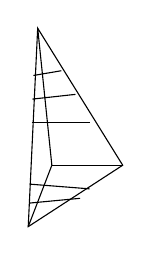
\begin{tikzpicture}[scale=1.2]
\draw(0,0)--(.1,2.1)--(1, .65)--cycle;
\draw(.1,2.1)--(.25,.65)--(0,0);\draw(.25,.65)--(1,.65);
\draw(.055,1.6)--(.35,1.65);\draw(.045,1.35)--(.5,1.4);
\draw(.035,1.1)--(.65,1.1);\draw(.015,.45)--(.65,.4);
\draw(.02,.25)--(.55,.3);
\end{tikzpicture}}
\diagram{\begin{tikzcd}A_{/a}\arrow[r]&A\end{tikzcd}}
\figure{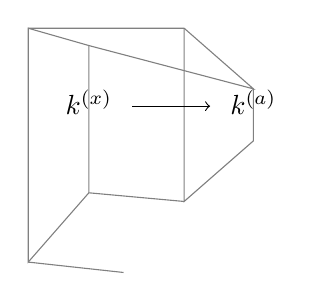
\begin{tikzpicture}[scale=1.1]
\draw[gray](0,0)--(.7,.8)--(.7,2.5)--(0,2.7)--cycle;
\draw[gray](0,2.7)--(1.8,2.7)--(2.6,2)--(.7,2.5);
\draw[gray](1.8,2.7)--(1.8,.7)--(2.6,1.4)--(2.6,2);
\draw[gray](.7,.8)--(1.8,.7);\draw[gray](0,0)--(1.1,-.12);
\node at(.7,1.85){$k^{(x)}$};\node at(2.6,1.85){$k^{(a)}$};
\draw[->](1.2,1.8)--(2.1,1.8);
\end{tikzpicture}}
\diagram{\begin{tikzcd}[column sep=small]
\unsure{x_M,y_M}\arrow[dd,bend right=15]&x&y\arrow[dl,bend left=12]\\
&k^{(x)}&\unsure{k^{(y)}}\\
f_!\underline{\operatorname{Hom}}(x,y)\arrow[r]&\unsure{k^{(\operatorname{Hom}(x,y))}|\operatorname{Hom}(k^{(x)},k^{(y)})}&
\end{tikzcd}}

\rotatebox{-90}{\begin{minipage}{24cm}
\[
K(\mathbb Z,n\qquad\operatorname{Symbin}^*(\qquad L.
\]
\diagram{\begin{tikzcd}[ampersand replacement=\&]
k[t]\arrow[r]\&k\langle t\rangle\\
k\arrow[u]\&
\end{tikzcd}}
\[
k\{P_n(t)\qquad \alpha t\qquad2\alpha
\]
\[
n!\,\unsure{P_n(t)}=t(t-1)\ \inserted{P}\,(t-n+1)
\]
\[
\frac{a(a-1)}{\deleted{\unsure{a}}2}\mathbin{\text{---}}\qquad\frac{t^2}{2}
\]
\[
x(x-1)\mathbin{\text{---}}(x-p+1)\qquad t(t-1)
\]
\[
\frac{x(x-1)}{2}=
\]
\deleted{$\unsure{x(t-1)=\frac{x}{p}}$}
\[
1+at+P(a)t^2
\]
\[
\unsure{1+bt+P(b)}
\]
\[
at+P(a)
\]
\[
(a+b)t+P(a+b)t^2
\]
\[
P(a+b)=P(a)+P(b)+ab
\]
$\mathbb Z\langle t\rangle$\qquad binomial

\figure{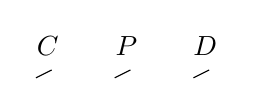
\begin{tikzpicture}
\node at(0,.4){$C$};\node at(1,.4){$P$};\node at(2,.4){$D$};
\draw(-.15,0)--(.05,.1);\draw(.85,0)--(1.05,.1);\draw(1.85,0)--(2.05,.1);
\end{tikzpicture}}
$a(b)$
\end{minipage}}

$\mathbb Z^{(a)}$

\rotatebox{90}{\begin{minipage}{27cm}
\diagram{$\begin{array}{lllllll}
\texttt{PPPPPPPPPPP}&\texttt{RRRRRRRRRRR}&\texttt{EEEEEEEEEEEE}&\texttt{DDDDDDDDD}&\texttt{OOOOOOOOOOOO}&\texttt{NN\ \ \ \ \ \ \ \ NN}&\texttt{TTTTTTTTTTTT}\\
\texttt{PPPPPPPPPPPP}&\texttt{RRRRRRRRRRRR}&\texttt{EEEEEEEEEEEE}&\texttt{DDDDDDDDDD}&\texttt{OOOOOOOOOOOO}&\texttt{NNN\ \ \ \ \ \ \ NN}&\texttt{TTTTTTTTTTTT}\\
\texttt{PP\ \ \ \ \ \ \ \ PP}&\texttt{RR\ \ \ \ \ \ \ \ RR}&\texttt{EE}&\texttt{DD\ \ \ \ \ \ \ DD}&\texttt{OO\ \ \ \ \ \ \ \ OO}&\texttt{NNNN\ \ \ \ \ \ NN}&\texttt{\ \ \ \ \ TT}\\
\texttt{PP\ \ \ \ \ \ \ \ PP}&\texttt{RR\ \ \ \ \ \ \ \ RR}&\texttt{EE}&\texttt{DD\ \ \ \ \ \ \ \ DD}&\texttt{OO\ \ \ \ \ \ \ \ OO}&\texttt{NN\ NN\ \ \ \ \ NN}&\texttt{\ \ \ \ \ TT}\\
\texttt{PP\ \ \ \ \ \ \ \ PP}&\texttt{RR\ \ \ \ \ \ \ \ RR}&\texttt{EE}&\texttt{DD\ \ \ \ \ \ \ \ DD}&\texttt{OO\ \ \ \ \ \ \ \ OO}&\texttt{NN\ \ NN\ \ \ \ NN}&\texttt{\ \ \ \ \ TT}\\
\texttt{PPPPPPPPPPPP}&\texttt{RRRRRRRRRRRR}&\texttt{EEEEEEEE}&\texttt{DD\ \ \ \ \ \ \ \ DD}&\texttt{OO\ \ \ \ \ \ \ \ OO}&\texttt{NN\ \ \ NN\ \ \ NN}&\texttt{\ \ \ \ \ TT}\\
\texttt{PPPPPPPPPPP}&\texttt{RRRRRRRRRRR}&\texttt{EEEEEEEE}&\texttt{DD\ \ \ \ \ \ \ \ DD}&\texttt{OO\ \ \ \ \ \ \ \ OO}&\texttt{NN\ \ \ \ NN\ \ NN}&\texttt{\ \ \ \ \ TT}\\
\texttt{PP}&\texttt{RR\ \ \ \ RR}&\texttt{EE}&\texttt{DD\ \ \ \ \ \ \ \ DD}&\texttt{OO\ \ \ \ \ \ \ \ OO}&\texttt{NN\ \ \ \ \ NN\ NN}&\texttt{\ \ \ \ \ TT}\\
\texttt{PP}&\texttt{RR\ \ \ \ \ RR}&\texttt{EE}&\texttt{DD\ \ \ \ \ \ \ \ DD}&\texttt{OO\ \ \ \ \ \ \ \ OO}&\texttt{NN\ \ \ \ \ \ NNNN}&\texttt{\ \ \ \ \ TT}\\
\texttt{PP}&\texttt{RR\ \ \ \ \ \ RR}&\texttt{EE}&\texttt{DD\ \ \ \ \ \ \ DD}&\texttt{OO\ \ \ \ \ \ \ \ OO}&\texttt{NN\ \ \ \ \ \ \ NNN}&\texttt{\ \ \ \ \ TT}\\
\texttt{PP}&\texttt{RR\ \ \ \ \ \ \ RR}&\texttt{EEEEEEEEEEEE}&\texttt{DDDDDDDDDD}&\texttt{OOOOOOOOOOOO}&\texttt{NN\ \ \ \ \ \ \ \ NN}&\texttt{\ \ \ \ \ TT}\\
\texttt{PP}&\texttt{RR\ \ \ \ \ \ \ \ RR}&\texttt{EEEEEEEEEEEE}&\texttt{DDDDDDDDD}&\texttt{OOOOOOOOOOOO}&\texttt{NN\ \ \ \ \ \ \ \ \ N}&\texttt{\ \ \ \ \ TT}
\end{array}$}
\begin{tabular}{l}
\texttt{****A END JOB 1282 PREDONT - CRAY OUTPUT - ROOM 6.48.16 PM 19 MAY 82 R6.PR1 SYS JES2 JOB 1282 END A****}\\
\texttt{****A END JOB 1282 PREDONT - CRAY OUTPUT - ROOM 6.48.16 PM 19 MAY 82 R6.PR1 SYS JES2 JOB 1282 END A****}\\
\texttt{****A END JOB 1282 PREDONT - CRAY OUTPUT - ROOM 6.48.16 PM 19 MAY 82 R6.PR1 SYS JES2 JOB 1282 END A****}\\
\texttt{****A END JOB 1282 PREDONT - CRAY OUTPUT - ROOM 6.48.16 PM 19 MAY 82 R6.PR1 SYS JES2 JOB 1282 END A****}\\
\texttt{****A END JOB 1282 PREDONT - CRAY OUTPUT - ROOM 6.48.16 PM 19 MAY 82 R6.PR1 SYS JES2 JOB 1282 END A****}\\
\texttt{****A END JOB 1282 PREDONT - CRAY OUTPUT - ROOM 6.48.16 PM 19 MAY 82 R6.PR1 SYS JES2 JOB 1282 END A****}
\end{tabular}
\end{minipage}}
\mspage{73}
\scanpage{75}
\diagram{\begin{tikzcd}
f:M\arrow[r]\arrow[dr,"\kappa_M"']&N\arrow[d,"\kappa_N"]\\
&\mathrm{ab}_k
\end{tikzcd}}
\deleted{$k$-additif compatible}
\inserted{appl. de catégories \unsure{$k$-additives|$k$-biadditives} augm.}

\deleted{Conditions}\qquad Conditions

(i) $H_i(M,f^*(y))=0\quad\forall y\text{ en }N\quad i>0$,
et $H_0(M,f^*(y))\xrightarrow{\simeq}H_0(N,y)$

\deleted{i.e. $f_!f^*y\longrightarrow y$}
\deleted{i.e. $f_!f^*y\longrightarrow y$}

(ii) $\forall G\text{ en }N^{\unsure{\flat|b}}$,
$LH_\bullet(M,f^*G)\xrightarrow{\simeq}LH_\bullet(N,G)$

(ii') \rule{3cm}{.4pt}\qquad $f_!f^*G\longrightarrow G$ est dans $W_N$

\deleted{(ii'') $\forall$}

(iii) (iii') avec $G$ dans $N$

(iv) $\forall G\text{ en }N_{\unsure{as|ab}}^{\unsure{\flat|b}}$,
$G\text{ asph}\Longrightarrow f^*G\text{ asph}$

iv') \rule{4cm}{.4pt}\qquad $G\text{ asph}\Longleftrightarrow f^*G\text{ asph}$

(v) \deleted{$\unsure{f^*}(W_N)=W$}\qquad
$W_N\subset f^{*-1}(W_M)$\quad i.e. $u\in W_N\Longrightarrow f^*u\in W_M$

(v')\quad\deleted{\unsure{(vi)}}\quad\deleted{$\unsure{f_*}$}\qquad
$W_N=f^{*-1}(W_M)$\quad $\text{---}\quad u\in W_M\Longleftrightarrow f^*u\in W_M$

(vi) \inserted{\uline{Ou}} (iv), et
\[
W_N^{-1}N^{\unsure{\flat|b}}\overset{\simeq}{\mathbin{\text{---}}}W_M^{-1}M^{\unsure{\flat|b}}.
\]

\diagram{\begin{tikzcd}[column sep=small,row sep=large]
&\deleted{\unsure{(i)}}\arrow[d,Rightarrow]&&\\
\left\{\vphantom{\begin{matrix}0\\0\\0\end{matrix}}\right.&
(ii)\arrow[r,Leftrightarrow]\arrow[d,Rightarrow]&(ii')&{}\\
&(iii)\arrow[r,Leftrightarrow]\arrow[d,Rightarrow]&(iii')\arrow[r,Leftrightarrow]&(i)\arrow[u,Rightarrow]\\
&(v')\arrow[d,Rightarrow]\arrow[dr,Rightarrow]&&\\
&(iv')\arrow[dr,Rightarrow]&(v)\arrow[d,Rightarrow]\arrow[uur,Rightarrow,bend right=24,"{\begin{array}{l}\text{Si }M,N\text{ asph. i.e.}\\\kappa_{M!}(1_M)\simeq k\\\kappa_{N!}(1_N)\simeq k\end{array}}"'{draw,ellipse,inner sep=2pt}]&\\
&&(iv)\arrow[uuur,Rightarrow,bend right=38,"{\begin{array}{l}\text{Si }M,N\text{ asph}\\\text{et en plus pour }x\text{ projectif en }N\\x\longrightarrow\kappa_N^*\kappa_{N!}x\quad\text{\uline{épi}}\end{array}}"'{draw,rectangle,rounded corners=3pt,inner sep=2pt}]&
\end{tikzcd}}

argument de résolution d'objets de $N^{\unsure{\flat|b}}$
par des \inserted{sommes d'} objets de $N$

(iv) $\Longrightarrow$ i)\qquad Soit $y\in N$, on a alors
$y\longrightarrow\kappa_N^*\kappa_{N!}(y)$ est dans $W_N$

(Cf Lemme ci-dessous)\quad\deleted{et est épi.}

donc via iv, si on app. $f^*$

\uline{Lemme}\qquad Donc a -
\deleted{$\unsure{f_!f^*\xi}\simeq f_!(1_M)\otimes$}
\[
f_!f^*(\xi)=f_!(1_M)\otimes_k\xi
\xrightarrow{\deleted{\unsure{\text{iso}}}}\xi
\]
\diagram{\begin{tikzcd}
f_!(x)\arrow[r]&f_!f^*f_!(x)\arrow[r]&f_!x
\end{tikzcd}}
\[
1_M\otimes f_!(x)
\]
\[
f^*y\longrightarrow\kappa_M^*(\kappa_{N!}y)
\]
\deleted{devient ds}\quad dans $W_M$\qquad
$f_!(1_M)\longrightarrow1_M$

\deleted{$L\unsure{f_{M!}}$}
\[
L\kappa_{M!}(f^*y)\xrightarrow[\deleted{\unsure{\xi}}]{\deleted{\simeq}}L\kappa_{N!}y
\]
OK
\figure{\begin{tikzpicture}
\draw(0,0)..controls(.4,2.3)and(.9,2.1)..(.9,.4)..controls(1.2,2.4)and(1.5,1.5)..(1.5,.2);
\draw(.9,.3)..controls(2,1.7)and(2.7,1.9)..(3.6,1.6)..controls(6,1.9)and(9.6,1.5)..(12,1.1);
\draw[->](3.2,1.6)..controls(6,1.6)and(10,1.8)..(13,1.2);
\draw[->](9,.4)..controls(9.6,-.1)and(12.8,.5)..(13,1.2);
\end{tikzpicture}}
\mspage{74}
\scanpage{76}
\deleted{SGA 7 Exposé $\overline{\underline{\mathrm{IX}}}$}
\figure{\begin{tikzpicture}
\draw(0,0)..controls(.4,-.05)and(.6,.1)..(.9,0)--(2,0)..controls(3,-.1)and(4,0)..(5,0)..controls(6,.1)and(6.5,-.05)..(7,0);
\draw[gray](-2,-1.2)--(2,2);\draw[gray](3,2)--(-1,-2)..controls(-1.4,-2.5)and(0,-1.6)..(2.5,-.1);
\draw[gray](4,1.4)--(2.4,-1.2)--(9.5,-.2);
\end{tikzpicture}}

$\bullet$ \deleted{Références à compléter dans la bibliographie.}

$\bullet$ $\mathcal M\quad1_M\text{ en }M\qquad
\kappa^*: \xi\longrightarrow1_M\otimes\xi$
admet adjoint à g. $\kappa_!$
\[
\mathrm{Ab}_k\mathbin{\text{---}}\mathcal M
\]
\deleted{$\kappa_!\kappa^*\xi\simeq\kappa_!(1_M)\otimes\xi
\xrightarrow{\alpha_\xi\ (\text{adj})}\xi$}

$\unsure{\beta_\xi}:$
\diagram{\begin{tikzcd}
\kappa_!\kappa^*(\xi)\arrow[r,dash,"\alpha_\xi"]&\xi\\
\kappa_!(1_M)\otimes\xi\arrow[u,"\simeq"]\arrow[r,"{\alpha_k\otimes\xi}"']&\xi\arrow[u,equal]
\end{tikzcd}}
\[
\alpha_k:\kappa_!(1_M)\mathbin{\text{---}}1_k
\]

\uline{Cor} Supposons que $\kappa_!(1_M)\xrightarrow{\alpha_k}1_k$,
alors $\kappa_!\kappa^*(\xi)\xrightarrow{\simeq}\xi$

i.e. $\kappa^*$ est pl. fid\par
$\kappa_!$ une localisation

\deleted{\uline{Cor} Supposons}
\deleted{NB}
\deleted{$\unsure{k}\ \kappa_!$ transforme projectifs en projectifs}
\deleted{donc $L\kappa_!$ adj.}

Supposons $M$ assez en proj. et
\[
L\kappa_!(1_M)\xrightarrow{\simeq}\kappa_!(1_M)\xrightarrow{\simeq}1_k
\]
Alors pour tout $x$ projectif en $M$, on a
\[
x\longrightarrow\kappa^*\kappa_!x\qquad\text{dans }W_M
\]
\deleted{$L_i\kappa_!x=0\text{ si }i>0,\quad
\unsure{L_i\kappa_!\kappa^*\xi=L_i}$}
\[
L\kappa_!\left(\underbrace{\kappa^*\kappa_!x}_{1_M\otimes\kappa_!x}\right)
\underset{\substack{\vert\\\text{car }\kappa_!x\text{ est}\\\text{projectif}}}{\simeq}
L\kappa_!(1_M)\otimes\kappa_!x
\]
\[
\simeq1_k\otimes\kappa_!x\simeq\kappa_!x
\]
\[
\simeq L\kappa_!x
\]
\mspage{75}
\scanpage{77}
$\mathcal M$ \deleted{$\unsure{\xi}$} cat. $k$-abélienne avec
\deleted{suffis} $\varinjlim$ et suff. en projectifs
\inserted{et syst. gén.}

$1_M$ tel que
\[
\mathrm{Ab}_k\longrightarrow\mathcal M\qquad
\kappa^*: \xi\longmapsto1_M\otimes_k\xi
\]
commute aux \deleted{produits} \inserted{$\varprojlim$}
i.e. admet un \uline{adjoint à gauche} $\kappa_!$
(alors qu'il admet un adj. à droite
$\kappa_*:a\longmapsto\operatorname{Hom}(1_M,a)$).
\deleted{Conditions}

Alors $\kappa_!$ transforme projectifs en projectifs.

\deleted{Supposons $\mathcal M=M^{\unsure{\flat|b}}$, alors les}

$\kappa^*$ foncteurs \inserted{$:\mathrm{Ab}_k\longrightarrow\mathcal M$, $k$-add}
qui ont un adjoint à gauche et à droite

i.e. qui \deleted{\unsure{ont} commutent aux $\varprojlim$}
commutent aux $\varprojlim$ et $\varinjlim$

Objets $1_M$ tels que

foncteurs $\kappa_!:\mathcal M\mathbin{\text{---}}\mathrm{Ab}_k$
qui commutent aux $\varinjlim$, et

dont l'adjoint \inserted{à dr.} commute aux $\varinjlim$ aussi.

Ex. $\mathcal M=M^{\unsure{\flat|b}}$:
foncteur $M\xrightarrow{\kappa_M}\mathrm{Ab}_k$ qui se factorise par
$\unsure{\mathrm{fab}_k}$

\uline{NB} $1_M:M^o\longrightarrow\mathrm{Ab}_k$
\deleted{\unsure{bien défini $\kappa_!$}}
\inserted{se factorise par $\mathrm{ab}_k$}

soit $\kappa'_M:M^o\longrightarrow\mathrm{ab}_k$,
ce dernier ``n'est autre que'' $\kappa_M^o$

Soit $x$ dans $M$, a-t-on
\[
x\longrightarrow\underbrace{\kappa^*\kappa_!x}_{1_M\otimes\kappa(x)}
\quad\text{épi}
\]
i.e. $\forall y$ dans $M^{\unsure{\flat|b}}$, a-t-on
\[
\begin{array}{c}
\operatorname{Hom}(1_M\otimes\kappa(x),\unsure{y|z})
\longrightarrow\operatorname{Hom}(x,z)\quad\text{mono}\\
\rotatebox{90}{$=$}\\
\operatorname{Hom}_k(\kappa(x),\operatorname{Hom}(1_M,z))\\
\rotatebox{90}{$=$}\\
\operatorname{Hom}(x,\underbrace{1_M\otimes\operatorname{Hom}(1_M,z)}_{f^*f_*z})
\end{array}
\]
\margin{$f^*f_*z\longrightarrow z\quad\text{mono ?}$}

\uline{Ex} $\mathcal M=\mathrm{Ab}_k\qquad1_M=X$ un $k$-module
la condition de commutation \inserted{de $X\otimes_k$} aux $\varprojlim$
signifie
$X$ plat de prés. finie i.e. $X$ proj. de t. f.
\[
M=\mathrm{ab}_k
\]
\[
\kappa^*(\xi)=X\otimes\xi,\qquad\kappa_!(x)=a\otimes\check X
\]
\[
x\longrightarrow\kappa^*(\kappa_!x)=a\otimes\check X\otimes X
\qquad\deleted{\unsure{donc}}\quad\text{épi}\Longleftrightarrow X\text{ de rg }\leq1
\]
\[
\kappa_!\kappa^*(\xi)=\check X\otimes X\otimes\xi\longrightarrow\xi
\qquad\text{mono}\Longleftrightarrow X\text{ de rg }\leq1
\]
\[
\kappa^*\kappa_*x=X\otimes\check X\otimes x\longrightarrow x
\qquad\text{mono}\Longleftrightarrow X\text{ de rg }\leq1
\]
\[
\xi\mathbin{\text{---}}\kappa_*\kappa^*\xi=\check X\otimes X\otimes\xi
\]
\mspage{76}
\scanpage{78}
SGA 7 Exposé $\overline{\underline{\mathrm{VIII}}}$
\figure{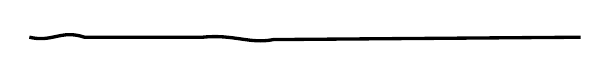
\begin{tikzpicture}
\draw[line width=1.2pt](0,0)..controls(.3,-.07)and(.4,.1)..(.7,0)--(2.2,0)..controls(2.6,.04)and(2.8,-.09)..(3.1,-.03)--(7,0);
\end{tikzpicture}}

$\bullet$ p 95. Cette dernière page est très serrée. Voir pour tirage photo-offset

\mspage{77}
\scanpage{79}
\[
0\longrightarrow x^{\unsure{a}}\longrightarrow x\longrightarrow j^*j_!x\mathbin{\text{---}}0
\]
\[
M\xrightarrow{\kappa}\mathrm{ab}_k
\]
\diagram{\begin{tikzcd}
M^o\arrow[r,leftrightarrow,"\kappa^o"]\arrow[rr,bend right=22,"\kappa'"']&\mathrm{ab}_k^o\arrow[r,"\vee"]&\mathrm{ab}_k
\end{tikzcd}}
\[
x\longrightarrow j^*j_!x\qquad\text{en }\underline M^{\deleted{\unsure{\flat}}}
\qquad(\text{car }1_M\in M)
\]
\[
\operatorname{Hom}_k(j_!x,\xi)\simeq\operatorname{Hom}_M(x,1_M\otimes\xi)
\]
\[
\operatorname{Hom}_k(j_!x,k)=(j_!x)^\vee=\operatorname{Hom}_M(x,1_M)
\]
\[
\boxed{j_!x=\operatorname{Hom}_{\unsure{M^\flat|M}}(x,1_M)^\vee}
\]
\margin{pour $x$ dans $M$\par
\deleted{si \unsure{Hom} les}\par
et $\operatorname{Hom}_M(x,1_M)$ proj. de t. f.}
\[
j'_!x=\operatorname{Hom}_M(x,1_M)
\]
\[
\overset{?}{\simeq}
\underbrace{\operatorname{Hom}_{M^o}(x^o,1_{M^o})^\vee}_{\operatorname{Hom}_M(1_{M^o},x)}
\]
\[
\operatorname{Hom}_M(x,1_M)\times\operatorname{Hom}_M(1_{M^o},a)
\xrightarrow{\text{dualité}}k
\]
\figure{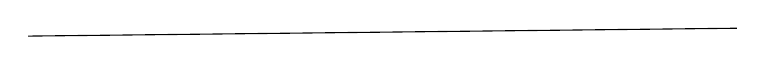
\begin{tikzpicture}\draw(0,0)--(9,.1);\end{tikzpicture}}
\[
\mathrm{ch}.(\mathrm{Ab}_k)\in\mathrm{Ch}.(\mathrm{Ab}_k)
\qquad\deleted{\unsure{\xi}}\ 1_k
\]
\[
\kappa=\underline H_0
\]
\margin{$\mathrm{Ch}_{\bullet}(\mathrm{Ab}_k)^o\simeq\mathrm{ch}^{\bullet}(\mathrm{Ab}_k)$}
\[
\kappa'=\underline H_0^\vee(L_.)=H^o(L_.^\vee)
\]
\mspage{78}
\scanpage{80}
\mspage{3}
centimètres de \unsure{longueur|longeur}, fendus longitudinalement au couteau pour que le\\
goût de l'aromate pénètre mieux dans l'eau environnante. Egalement, on\\
peut ajouter dans le pot quelques piments frais ou secs entiers, ils con-\\
tribuent à la conservation du Kimchi et lui donnent un goût un peu plus\\
corsé, sans risquer d'avoir un effet irritant comme la poudre de piment.\\
Quant à l'ail (et toujours pour le Kimchi à l'eau), chaque gousse épluchée\\
est coupée en deux (ou trois, si elle est grosse), et mise à infuser dans\\
le pot, avec les autres aromates. Les aromates ne sont écrasées au mortier\\
que pour le Kimchi ``sans eau''.

La quantité de sel et d'aromates à ajouter pour un pot de Kimchi est\\
réglé au goût, qui doit être engageant, ni trop fort ni trop faible. Il\\
vaut mieux en mettre au début trop peu que trop, quitte à en rajouter le\\
lendemain, ce qui n'offre pas de difficulté. Un Kimchi fortement salé ou\\
épicé pourra être délicieux, à condition qu'il soit servi comme condiment\\
(pour accompagner pommes de terre ou céréales notamment), plutôt que comme\\
plat de légumes.

3.\quad Le matériel nécessaire pour la préparation du Kimchi (mis à part les\\
ingrédients dont il vient d'être question) est des plus simples. Le plus\\
important est le pot en terre ou en grès - il est bon d'en avoir un assor-\\
timent de tailles différentes, suivant les quantités de légumes dont on\\
dispose d'un cas à l'autre. En Corée les pots familiaux de cents ou deux\\
cent litres sont pratique courante et ils y sont peu coûteux - pour notre\\
usage des pots entre trois et vingt litres feront sans doute l'affaire, on\\
en trouve dans le commerce sans trop de mal (quitte à faire une commande au\\
besoin), pour des prix variant suivant la taille, de trente à 200 frs.\\
Il faut aussi disposer de couvercles pour les pots, qui ne doivent jamais\\
rester ouverts quand ils sont en service. D$\underset{\unsure{e}}{\overset{-}{\mathrm e}}$s assiettes font généralement\\
l'affaire, et sont préférables à des planchettes en bois, qui favorisent\\
l'apparition de moisissures. Il est bon quand on prépare le Kimchi de\\
choisir un pot de taille approprié, de façon qu'il soit à peu près rempli\\
et non à demi plein seulement, pour éviter un grand contact d'air.

Pour puiser le Kimchi dans le\unsure{x|s} pot, il convient d'utiliser une\\
spatule ou cuillère en bois pour le Kimchi sans eau, une louche (en bois\\
de préférence) pour le Kimchi à l'eau. Cuillère et louche doivent être\\
propres \uline{et sèches} (les essuyer après lavage !), sous peine d'introduire\\
des fermentations parasites dans le pot et de faire ``tourner'' le Kimchi.\\
Ne pas utiliser la même cuillère ou louche pour plusieurs pots de Kimchi,\\
sans l'avoir lavée et séchée après chaque usage. Eviter de prendre du Kim-\\
chi avec la main dans le pot, sauf si elle vient d'être lavée. Quand on a
\mspage{79}
\scanpage{81}
\[
\left\{\begin{array}{l}
\kappa_!=H_0(M,-)
\overset{\substack{\text{pour arg. dans }M\\
\text{(plus gén\textsuperscript{t}, tels que }\operatorname{Hom}(x,1_M)\text{ ds }\mathrm{ab}_k)}}{=}
\operatorname{Hom}(-,1_M)^\vee\\[3pt]
\kappa^*=1_M\otimes_k-\\[3pt]
\kappa_*=\operatorname{Hom}(1_M,-)=H^o(M,-)
\end{array}\right.
\]

$J$ dans $M^{\unsure{\flat|b}}$, avec structure d'algèbre augmentée vers
\inserted{(pas néc comm. ni assoc.)}
$1_M$, avec deux hom $1_M\rightrightarrows J$ qui relèvent
l'augmentation [et tels que
$1_M\times1_M\mathbin{\text{---}}J$ \uline{soit injectif}].

\diagram{\begin{tikzcd}
J\arrow[r,"\varepsilon"]&1_M\\
1_M\times1_M\arrow[u,hook,"{(\delta_0,\delta_1)}"]
\end{tikzcd}}

Supposons que $J\longrightarrow1_M$
soit dans $W_M$, et le reste
par produit tensoriel par $\forall x$ dans $M^{\unsure{\flat|b}}$
(on dit que c'est dans $UW_M$). Considérons
un \unsure{autre} \deleted{de \unsure{s. système}} \inserted{objet} $J'$
(qui n'a pas de multiplication) avec
\deleted{$\unsure{\varepsilon}$} augm $\varepsilon'$ et deux co-augm.
$\delta'_0,\delta'_1$ (``intervalles'' dans $M^{\unsure{\flat|b}}$) et
\[
J'\longrightarrow J^{\unsure{\deleted{'}}}
\]
compatible avec les augmentations et
\inserted{bi-}co-augmentations. Je dis qu'alors \deleted{si $J$}
\[
\varepsilon':J'\mathbin{\text{---}}1_M\quad\text{est aussi dans }UW_M
\]
\diagram{\begin{tikzcd}
J\otimes x\arrow[r]\arrow[d]&J'\otimes x\arrow[d]\\
x&x
\end{tikzcd}}

\margin{On suppose que $\delta_0$ joue le rôle d'une unité
et $\delta_1$ \unsure{celui d'un élément absorbant}
\[
\underbrace{1_M\otimes J}_{\simeq J}
\xrightarrow{\delta_0\times\mathrm{id}_J}J\otimes J\xrightarrow{\pi}J
\]
est l'identité, et
$\pi\cdot(\delta_1\times\mathrm{id}_J)$ est le composé de
$\delta_1\varepsilon$.}
\mspage{80}
\scanpage{82}
\mspage{4}
pris du Kimchi dans un saladier et qu'il en reste après le repas, ne pas\\
le remettre dans le pot, mais le garder pour le terminer à l'un des repas\\
suivants. Il se gardera plusieurs jours dans le saladier sans problème,\\
alors que le Kimchi dans le pot doit se garder plusieurs semaines, voire\\
plusieurs mois.

Comme matériel pour la préparation proprement dite, il faut prévoir\\
une planche pour découper les légumes, un grand couteau de cuisine, plu-\\
sieurs sceaux ou grandes cuvettes pour le lavage \unsure{et} le malaxage des légumes,\\
un ou deux grands tamis ronds en paille ou bambou tressés pour égoutter -\\
on en trouve d'importation chinoise pour vingt à trente francs. J'en ai deux,\\
et même en dehors des moments de préparation du Kimchi, ils me servent pra-\\
tiquement tous les jours, pour laver des légumes ou des céréales, comme\\
\deleted{panier} corbeille à fruits et à légumes etc. Enfin, pour les Kimchis sans\\
eau, il faut un mortier avec pilon pour écraser ensemble le sel et les aro-\\
mates.

4.\quad La préparation et la conservation du Kimchi est chose des plus simples,\\
et il n'y a aucun problème dès qu'on lui consacre un minimum d'intelligence\\
et de soin. (Celui qui n'est pas disposé à faire ce minimum d'investissement\\
fera mieux de se nourrir de conserves ...) La première et principale exigean\\
-ce est la propreté. Tous les instruments utilisés pour la préparation \unsure{et|ou}\\
l'utilisation du Kimchi doivent être propres. Plus particulièrement, au\\
moment de la préparation, le pot qu'on s'apprête à utiliser doit être lavé\\
soigneusement tant intérieurement qu'extérieurement, et séché intérieurement\\
avec un torchon propre. De même pour les sceaux et cuvettes, la planche à\\
découper etc. La table de travail doit être nette de tout objet étranger à\\
la préparation du Kimchi, et propre. Les mains et bras sont propres, et\\
tout particulièrement pour le malaxage des légumes avec les aromates (cas du\\
Kimchi sans eau). On évitera de remplir le pot à ras-bord, pour que l'assi-\\
ette-couvercle ne soit pas au contact du Kimchi, et pour éviter aussi que le\\
pot ne déborde à la suite du ``travail'' du Kimchi dans les premiers jours.

Dans les jours qui suivent la préparation du Kimchi, alors que la\\
fermentation s'amorce, il est bon de surveiller le déroulement, en remuant\\
le Kimchi à l'eau pour faire replonger les légumes montés à la surface\\
et éviter qu'ils ne se dessèchent ou ne moisissent, ou tasser (avec une\\
cuillère en bois ou une louche, ou à la main lavée au préalable) le Kimchi\\
sans eau, de sorte que le jus passe au dessus du Kimchi, dont la partie supé-\\
\unsure{rièure|rieure} restera humide. Il est bon de le faire tous les un ou deux jours.\\
U$\underset{\unsure{v}}{\overset{\unsure{-}}{\mathrm n}}$e fois que le Kimchi est bon pour la consommation, l'usage régulier du\\
Kimchi suffit à garantir en principe une bonne continuation du processus de
\mspage{81}
\scanpage{83}
\mspage{3}
centimètres de \unsure{longueur|longeur}, fendus longitudinalement au couteau pour que le\\
goût de l'aromate pénètre mieux dans l'eau environnante. Egalement, on\\
peut ajouter dans le pot quelques piments frais ou secs entiers, ils con-\\
tribuent à la conservation du Kimchi et lui donnent un goût un peu plus\\
corsé, sans risquer d'avoir un effet irritant comme la poudre de piment.\\
Quant à l'ail (et toujours pour le Kimchi à l'eau), chaque gousse épluchée\\
est coupée en deux (ou trois, si elle est grosse), et mise à infuser dans\\
le pot, avec les autres aromates. Les aromates ne sont écrasées au mortier\\
que pour le Kimchi ``sans eau''.

La quantité de sel et d'aromates à ajouter pour un pot de Kimchi est\\
réglé au goût, qui doit être engageant, ni trop fort ni trop faible. Il\\
vaut mieux en mettre au début trop peu que trop, quitte à en rajouter le\\
lendemain, ce qui n'offre pas de difficulté. Un Kimchi fortement salé ou\\
épicé pourra être délicieux, à condition qu'il soit servi comme condiment\\
(pour accompagner pommes de terre ou céréales notamment), plutôt que comme\\
plat de légumes.

3.\quad Le matériel nécessaire pour la préparation du Kimchi (mis à part les\\
ingrédients dont il vient d'être question) est des plus simples. Le plus\\
important est le pot en terre ou en grès - il est bon d'en avoir un assor-\\
timent de tailles différentes, suivant les quantités de légumes dont on\\
dispose d'un cas à l'autre. En Corée les pots familiaux de cents ou deux\\
cent litres sont pratique courante et ils y sont peu coûteux - pour notre\\
usage des pots entre trois et vingt litres feront sans doute l'affaire, on\\
en trouve dans le commerce sans trop de mal (quitte à faire une commande au\\
besoin), pour des prix variant suivant la taille, de trente à 200 frs.\\
Il faut aussi disposer de couvercles pour les pots, qui ne doivent jamais\\
rester ouverts quand ils sont en service. D$\underset{\unsure{e}}{\overset{-}{\mathrm e}}$s assiettes font généralement\\
l'affaire, et sont préférables à des planchettes en bois, qui favorisent\\
l'apparition de moisissures. Il est bon quand on prépare le Kimchi de\\
choisir un pot de taille approprié, de façon qu'il soit à peu près rempli\\
et non à demi plein seulement, pour éviter un grand contact d'air.

Pour puiser le Kimchi dans le\unsure{x|s} pot, il convient d'utiliser une\\
spatule ou cuillère en bois pour le Kimchi sans eau, une louche (en bois\\
de préférence) pour le Kimchi à l'eau. Cuillère et louche doivent être\\
propres \uline{et sèches} (les essuyer après lavage !), sous peine d'introduire\\
des fermentations parasites dans le pot et de faire ``tourner'' le Kimchi.\\
Ne pas utiliser la même cuillère ou louche pour plusieurs pots de Kimchi,\\
sans l'avoir lavée et séchée après chaque usage. Eviter de prendre du Kim-\\
chi avec la main dans le pot, sauf si elle vient d'être lavée. Quand on a
\mspage{82}
\scanpage{84}
\diagram{\begin{tikzcd}
x\arrow[rr,equal]\arrow[dr,shift left=2pt]\arrow[dr,shift right=2pt]&&x\arrow[dr,shift left=2pt]\arrow[dr,shift right=2pt]&\\
&I_x\arrow[rr]\arrow[d]&&I'_x\arrow[d]\\
&x\arrow[rr,"="]&&x
\end{tikzcd}}
\margin{$I_x\times$}
\figure{\begin{tikzpicture}
\draw(0,0)--(3,.1)..controls(4,.35)and(4.6,.3)..(5,.4)..controls(5.2,1.2)and(6,1.65)..(7.6,1.65)--(7.6,3.3);
\draw(5,.4)--(5,1.2)..controls(5.1,1.55)and(6.9,1.7)..(7.6,1.65);
\draw(5,.4)..controls(5.4,1.6)and(6.8,1.8)..(7.6,1.65);
\end{tikzpicture}}

\diagram{\begin{tikzcd}
&&k&\\
0\arrow[r,dash]&k\arrow[r]&k\times k\arrow[u,"\varepsilon"]\arrow[r,dash]&0
\end{tikzcd}}
\[
\underbrace{\qquad k\longrightarrow k\times k\qquad}_{\substack{\deleted{\unsure{\Delta^1_k}}\\\delta^1}}
\]
\[
\mathbf1\qquad\deleted{\unsure{\xi}}\quad\mathbf K
\]
\diagram{\begin{tikzcd}[column sep=large]
1_M&&\lambda^*(1_k)&\\
J\arrow[u,"\varepsilon"]\arrow[rr,rightsquigarrow]&&\lambda^*(\delta^1)\arrow[u]\arrow[r]&1_M\\
1_M\times1_M\arrow[u]&&\lambda^*(1_{\unsure{M|k}})\times\lambda^*(1_k)\arrow[u]
\end{tikzcd}}
\diagram{\begin{tikzcd}[column sep=large]
\lambda_!(1_M)\arrow[r,"{\alpha\ (\text{adj})}"]&1_k\\
\lambda_!J\arrow[u,"{\lambda_!(\varepsilon)}"]\arrow[r,"{\underbrace{\delta_0\alpha\lambda_!\varepsilon}_{\beta}}"']&\underline{\delta^1}\arrow[u]\\
\lambda_!1_M\arrow[u,shift left=2pt,"{\lambda_!(\delta_0)}"]\arrow[u,shift right=2pt,"{\lambda_!(\delta_1)}"']\arrow[r,"\alpha"']&1_k\arrow[u,shift left=2pt]\arrow[u,shift right=2pt]
\end{tikzcd}}

\[
-\qquad\underbrace{\delta_0\alpha\lambda_!(\varepsilon)}_{\beta}\lambda_!(\delta_0)
=\delta_0\alpha\lambda_!(\underbrace{\varepsilon\delta_0}_{\mathrm{id}})
=\delta_0\alpha\qquad\text{OK}
\]
\[
\delta_0\alpha\lambda_!(\varepsilon)\lambda_!(\delta_1)
=\delta_0\alpha\underline{\lambda_!(\varepsilon\delta_1)}
=\delta_0\alpha
\]

\diagram{\begin{tikzcd}
0\arrow[r,dash]&k\arrow[r]&k\unsure{\times|+}k\arrow[r,dash]&0\\
L_{\unsure{2}}\arrow[r]&L_{\unsure{1}}\arrow[r]\arrow[u]&L_0\arrow[u]\arrow[r,dash]&0
\end{tikzcd}}
\diagram{\begin{tikzcd}
L_{\unsure{1}}\arrow[r]&L_0\arrow[r,shift left=2pt,"\delta_0"]\arrow[r,shift right=2pt,"\delta_1"']&k
\end{tikzcd}}
\deleted{$\delta_0\unsure{H|HL}$}\qquad\deleted{$\delta_0d_1$}

$\delta_0-\delta_1$ se factorise par $H_0(L_.)$
\figure{\begin{tikzpicture}\draw(0,0)--(.7,0)..controls(1.1,0)and(1.4,0)..(1.5,-.4)--(1.5,-1.2);\end{tikzpicture}}

\diagram{\begin{tikzcd}[column sep=large]
1_M\arrow[r,"\alpha"]\arrow[d,"\varepsilon"]&\lambda^{\unsure{*|\prime}}(1_k)\arrow[d,shift left=2pt]\\
J\arrow[r,"\beta"]&\lambda^{\unsure{*|\prime}}(\underline{\delta^1})\arrow[u,shift left=2pt]\\
1_M\arrow[u,shift left=2pt,"\delta_0"]\arrow[u,shift right=2pt,"\delta_1"']\arrow[r,"\alpha"']&\lambda^{\unsure{*|\prime}}(1_k)\arrow[u,shift left=2pt]\arrow[u,shift right=2pt]
\end{tikzcd}}
\[
\beta\delta_0=\delta_0\alpha\qquad
\beta\delta_1=\delta_1\alpha
\]
\mspage{83}
\scanpage{85}
\mspage{4}
pris du Kimchi dans un saladier et qu'il en reste après le repas, ne pas\\
le remettre dans le pot, mais le garder pour le terminer à l'un des repas\\
suivants. Il se gardera plusieurs jours dans le saladier sans problème,\\
alors que le Kimchi dans le pot doit se garder plusieurs semaines, voire\\
plusieurs mois.

Comme matériel pour la préparation proprement dite, il faut prévoir\\
une planche pour découper les légumes, un grand couteau de cuisine, plu-\\
sieurs sceaux ou grandes cuvettes pour le lavage \unsure{et} le malaxage des légumes\\
un ou deux grands tamis ronds en paille ou bambou tressés pour égoutter -\\
on en trouve d'importation chinoise pour vingt à trente francs. J'en ai de\unsure{u}\\
et même en dehors des moments de préparation du Kimchi, ils me servent pra\unsure{-}\\
tiquement tous les jours, pour laver des légumes ou des céréales, comme\\
\deleted{panier} corbeille à fruits et à légumes etc. Enfin, pour les Kimchis sans\\
eau, il faut un mortier avec pilon pour écraser ensemble le sel et les aro-\\
mates.

4.\quad La préparation et la conservation du Kimchi est chose des plus \unsure{simples}\\
et il n'y a aucun problème dès qu'on lui consacre un minimum d'intelligence\\
et de soin. (Celui qui n'est pas disposé à faire ce minimum d'investissement\\
fera mieux de se nourrir de conserves ...) La première et principale exigean\\
-ce est la propreté. Tous les instruments utilisés pour la préparation \unsure{et|ou}\\
l'utilisation du Kimchi doivent être propres. Plus particulièrement, au\\
moment de la préparation, le pot qu'on s'apprête à utiliser doit être lavé\\
soigneusement tant intérieurement qu'extérieurement, et séché intérieurement\\
avec un torchon propre. De même pour les sceaux et cuvettes, la planche à\\
découper etc. La table de travail doit être nette de tout objet étranger à\\
la préparation du Kimchi, et propre. Les mains et bras sont propres, et\\
tout particulièrement pour le malaxage des légumes avec les aromates (cas du\\
Kimchi sans eau). On évitera de remplir le pot à ras-bord, pour que l'assi\unsure{-}\\
ette-couvercle ne soit pas au contact du Kimchi, et pour éviter aussi que le\\
pot ne déborde à la suite du ``travail'' du Kimchi dans les premiers jours.

Dans les jours qui suivent la préparation du Kimchi, alors que la\\
fermentation s'amorce, il est bon de surveiller le déroulement, en remuant\\
le Kimchi à l'eau pour faire replonger les légumes montés à la surface\\
et éviter qu'ils ne se dessèchent ou ne moisissent, ou tasser (avec une\\
cuillère en bois ou une louche, ou à la main lavée au préalable) le Kimchi\\
sans eau, de sorte que le jus passe au dessus du Kimchi, dont la partie supé-\\
\unsure{rièure|rieure} restera humide. Il est bon de le faire tous les un ou deux jours.\\
U$\underset{\unsure{v}}{\overset{\unsure{-}}{\mathrm n}}$e fois que le Kimchi est bon pour la consommation, l'usage régulier du\\
Kimchi suffit à garantir en principe une bonne continuation du processus de
\mspage{84}
\scanpage{86}
\diagram{\begin{tikzcd}
e&j^*(e)\\
I\arrow[u]\arrow[r,dash]&j^*\Delta^1\arrow[u]\\
e\arrow[u,shift left=2pt]\arrow[u,shift right=2pt]\arrow[r]&j^*(e)\arrow[u,shift left=2pt]\arrow[u,shift right=2pt]
\end{tikzcd}}
\diagram{\begin{tikzcd}
j_!I\arrow[r]&\Delta^1\\
j_!e\arrow[u,shift left=2pt]\arrow[u,shift right=2pt]\arrow[r]&e\arrow[u,shift left=2pt]\arrow[u,shift right=2pt]
\end{tikzcd}}
\[
j_!(e)\longrightarrow
\]
\diagram{\begin{tikzcd}
&0\arrow[r,dash]&k\arrow[r,dash]&0\\
0\arrow[r,dash]&k\arrow[r,dash]&k\times k\arrow[u]\arrow[r,dash]&0
\end{tikzcd}}
\[
k
\]
\deleted{$\lambda_!1_M$}
\diagram{\begin{tikzcd}
l_{\unsure{2|1}}\arrow[r]&l_1\arrow[r,dash]&l_0\arrow[r,dash]&0\\
L_{\unsure{2|n}}\arrow[u]\arrow[r]&L_1\arrow[u]\arrow[r]&L_0\arrow[u]\arrow[r,dash]&0
\end{tikzcd}}
\figure{\begin{tikzpicture}\draw(0,0)..controls(.7,.7)and(1.2,1.6)..(1.5,2.5);\end{tikzpicture}}
\diagram{\begin{tikzcd}
l_.\arrow[r,"{\alpha\ \text{qu'is}}"]&k\\
L_.\arrow[u]\arrow[r]&\underline{\delta^1}\arrow[u]\\
l_.\arrow[u,shift left=2pt]\arrow[u,shift right=2pt]\arrow[r,"\alpha","\text{qu'is}"']&k\arrow[u,shift left=2pt]\arrow[u,shift right=2pt]
\end{tikzcd}}

\deleted{$\unsure{\Theta}$}
\diagram{\begin{tikzcd}
L_.^{\unsure{\flat|b}}\arrow[r,"{u\ ?}"]&\unsure{\text{\textcircled{H}}|\Theta}=\underline{\delta^1}^{\unsure{\flat|b}}\\
l_.\arrow[u]\arrow[r,"\alpha"]&k\arrow[u]
\end{tikzcd}}
\diagram{\begin{tikzcd}
0\arrow[r,dash]&k\arrow[r,dash,"\simeq"]&k\arrow[r,dash]&0\\
L_{\unsure{2|n}}^{\unsure{\flat|b}}\arrow[r,dash]\arrow[d]&L_1^{\unsure{\flat|b}}\arrow[u]\arrow[r,"\text{surj}"']\arrow[d]&L_0^{\unsure{\flat|b}}\arrow[u,"u"]\arrow[r,dash]\arrow[d]&0\\
l_{\unsure{2|n}}\arrow[r,dash]&l_1\arrow[r,dash]&l_0\arrow[r,dash]\arrow[dr]&0\\
&&&k
\end{tikzcd}}
\margin{$L_0^{\unsure{\flat|b}}\longrightarrow k$}
\diagram{\begin{tikzcd}
0\arrow[r,dash]&k\arrow[r,dash]&k\arrow[r,dash]&{}\\
&0\arrow[r,dash]&k\arrow[u]\arrow[r,dash]&{}
\end{tikzcd}}
\[
\left\{\begin{array}{l}
1_M\longleftarrow J\quad\text{\unsure{univ\textsuperscript{t}} str. acycl.}\\
\deleted{\lambda_{0!}(1_M)\longrightarrow\lambda_0}\quad
J/1_M\text{ projectif, ou seulement }
\operatorname{Ext}^1(\lambda_{0!}(J/1_M),k)=0
\end{array}\right.
\]
\mspage{85}
\scanpage{87}
\rotatebox{180}{\begin{minipage}{\textwidth}
\mspage{3}
centimètres de \unsure{longueur|longeur}, fendus longitudinalement au couteau pour que le\\
goût de l'aromate pénètre mieux dans l'eau environnante. Egalement, on\\
peut ajouter dans le pot quelques piments frais ou secs entiers, ils con-\\
tribuent à la conservation du Kimchi et lui donnent un goût un peu plus\\
corsé, sans risquer d'avoir un effet irritant comme la poudre de piment.\\
Quant à l'ail (et toujours pour le Kimchi à l'eau), chaque gousse épluchée\\
est coupée en deux (ou trois, si elle est grosse), et mise à infuser dans\\
le pot, avec les autres aromates. Les aromates ne sont écrasées au mortier\\
que pour le Kimchi ``sans eau''.

\figure{\begin{tikzpicture}\draw(0,0)--(0,.25);\end{tikzpicture}}
La quantité de sel et d'aromates à ajouter pour un pot de Kimchi est\\
réglé au goût, qui doit être engageant, ni trop fort ni trop faible. Il\\
vaut mieux en mettre au début trop peu que trop, quitte à en rajouter le\\
lendemain, ce qui n'offre pas de difficulté. Un Kimchi fortement salé ou\\
épicé pourra être délicieux, à condition qu'il soit servi comme condiment\\
(pour accompagner pommes de terre ou céréales notamment), plutôt que comme\\
plat de légumes.

3.\quad Le matériel nécessaire pour la préparation du Kimchi (mis à part les\\
ingrédients dont il vient d'être question) est des plus simples. Le plus\\
important est le pot en terre ou en grès - il est bon d'en avoir un assor-\\
timent de tailles différentes, suivant les quantités de légumes dont on\\
dispose d'un cas à l'autre. En Corée les pots familiaux de cents ou deux\\
cent litres sont pratique courante et ils y sont peu coûteux - pour notre\\
usage des pots entre trois et vingt litres feront sans doute l'affaire, on\\
en trouve dans le commerce sans trop de mal (quitte à faire une commande au\\
besoin), pour des prix variant suivant la taille, de trente à 200 frs.\\
Il faut aussi disposer de couvercles pour les pots, qui ne doivent jamais\\
rester ouverts quand ils sont en service. D$\underset{\unsure{e}}{\overset{-}{\mathrm e}}$s assiettes font généralement\\
l'affaire, et sont préférables à des planchettes en bois, qui favorisent\\
l'apparition de moisissures. Il est bon quand on prépare le Kimchi de\\
choisir un pot de taille approprié, de façon qu'il soit à peu près rempli\\
et non à demi plein seulement, pour éviter un grand contact d'air.

Pour puiser le Kimchi dans le\unsure{x|s} pot, il convient d'utiliser une\\
spatule ou cuillère en bois pour le Kimchi sans eau, une louche (en bois\\
de préférence) pour le Kimchi à l'eau. Cuillère et louche doivent être\\
propres \uline{et sèches} (les essuyer après lavage !), sous peine d'introduire\\
des fermentations parasites dans le pot et de faire ``tourner'' le Kimchi.\\
Ne pas utiliser la même cuillère ou louche pour plusieurs pots de Kimchi,\\
sans l'avoir lavée et séchée après chaque usage. Eviter de prendre du Kim-\\
chi avec la main dans le pot, sauf si elle vient d'être lavée. Quand on a
\end{minipage}}
\mspage{86}
